\documentclass{article}
\usepackage[utf8]{inputenc}
\usepackage{amsmath}
\usepackage{amssymb}
\usepackage{graphicx}
\usepackage{tabularx}
\usepackage{booktabs}
\usepackage{caption}
\usepackage[english]{babel}
\usepackage{setspace}
\usepackage{geometry}
\usepackage{float}
\usepackage{url}
\usepackage[justification=centering]{caption}

% APA style formatting
\geometry{a4paper, margin=1in}
\setstretch{1.5}
\captionsetup[table]{labelfont=bf, justification=raggedright, singlelinecheck=false}
\captionsetup[figure]{font=small, labelfont=bf, justification=raggedright, singlelinecheck=false}

\title{ Machine Learning for Customer Churn Prediction}
\author{Nelson David Posso Suarez \\ Javier Alejandro Penagos Hernandez \\ Nicolas Castro Rivera }
\date{}

\begin{document}

\maketitle


\section{Executive Summary }
Customer Churn is a problem about customer discontinue a company's services or products. Machine learning techniques can be applied with purpose of predict if a customer 
has probability of be churn, this information can help the company to take decisions for not lost clients. This work search explore different machine learning techniques
to compare and get the best approach to solve this problem. 

\section{Dataset Download and Integrity Verification}

\subsection{Dataset Source and Acquisition}
The Telco Customer Churn dataset was obtained from the public Kaggle page published by 
BlastChar and identified as originating from IBM Sample Data Sets. To reproduce the setup, 
download the complete \path{WA_Fn-UseC_-Telco-Customer-Churn.csv} 
file from \url{https://www.kaggle.com/datasets/blastchar/telco-customer-churn} and 
place it at \path{data/WA_Fn-UseC_-Telco-Customer-Churn.csv}. 
The Kaggle page does not specify a standard open-source license; this project uses the data 
for academic learning and analysis and acknowledges its source and original authors.

\subsection{Dataset Characteristics}
The CSV is 977,501 bytes (approximately 977.5 KB) and contains 7,043 customer records and 21 columns: 20 customer and service features, plus the binary \texttt{Churn} target. It has 1,869 \texttt{Yes} and 5,174 \texttt{No} records, indicating class imbalance.

\subsection{Integrity Verification}
The provider does not supply an official checksum. To calculate the SHA-256 hash of the local project copy, run \path{python src/w1_supervized_learning/dataset_info/checksum.py} from the repository root. The script reads the CSV under \path{data/} and prints its checksum:

\begin{center}
\small\texttt{88BE4B93FBE0CC83421AF1C503794C97C342ECA914C1576DB7C276E61D61358A}
\end{center}

This value is a local reference because Kaggle does not provide an official checksum for comparison. To generate a structured dataset report, run \path{python src/w1_supervized_learning/dataset_info/dataset_info.py} from the repository root. It prints JSON with the file size, row and column counts, samples per \texttt{Churn} class, each column's data type and missing-value count, and numeric feature ranges. Both scripts use the Telco CSV by default; a different file can be supplied with \path{--csv}.


\section{Exploratory Data Analysis (EDA)}

This section explore the data, explain what represents each feature and respective type, 
the proportion in the values of numerical and categorical features, 
the relation between each feature with the target and visual representation of statistics obtained.
\\All process in this section can be explore in EDA notebook. 

\begin{table}[H]
\centering
\renewcommand{\arraystretch}{1.3}
\begin{tabularx}{\textwidth}{|l|X|l|}
\hline
\textbf{Feature} & \textbf{Description} & \textbf{Data type} \\ \hline
customerID & Unique value that identify a customer & \texttt{str} \\ \hline
gender & Determines whether customer is Male or Female & \texttt{str} \\ \hline
SeniorCitizen & Determines whether a person is citizen or not & \texttt{int64} \\ \hline
Partner & Determines whether person has partner & \texttt{str} \\ \hline
Dependents & Determines whether customer has a dependent & \texttt{str} \\ \hline
tenure & Number of months has stayed with the company & \texttt{int64} \\ \hline
PhoneService & Whether customer has phone service & \texttt{str} \\ \hline
MultipleLines & Whether the customer has multiple lines, or one, or does not have phone service & \texttt{str} \\ \hline
InternetService & Internet service provider (Fiber optic, DSL or no) & \texttt{str} \\ \hline
OnlineSecurity & Whether customer has online security, or not, or does not have internet service & \texttt{str} \\ \hline
OnlineBackup & Whether customer has online backup, or not, or does not have internet service & \texttt{str} \\ \hline
DeviceProtection & Whether customer has device protection, or not, or does not have internet service & \texttt{str} \\ \hline
TechSupport & Whether customer has tech support, or not, or does not have internet service & \texttt{str} \\ \hline
StreamingTV & Whether customer has streaming tv, or not, or does not have internet service & \texttt{str} \\ \hline
StreamingMovies & Whether customer has streaming movies, or not, or does not have internet service & \texttt{str} \\ \hline
Contract & Contract term duration (Month-to-month, One year, Two year) & \texttt{str} \\ \hline
PaperlessBilling & Whether customer has paperless billing or not & \texttt{str} \\ \hline
PaymentMethod & Payment method (Electronic check, Mailed check, Bank transfer (automatic), Credit card) & \texttt{str} \\ \hline
MonthlyCharges & Value paid by customer monthly & \texttt{float64} \\ \hline
TotalCharges & Total value paid by customer & \texttt{str} \\ \hline
Churn & Whether the customer churned or not, stopped using the service last month. & \texttt{str} \\ \hline
\end{tabularx}
\caption{\centering Dataset features description}
\label{tab:features}
\end{table}

\subsection{Target Distribution}
Of the 7,043 customers, 5,174 (73.46\%) stayed and 1,869 (26.54\%) churned. The majority-to-minority ratio is 2.77:1, so the target is moderately imbalanced. The class counts are summarized in Figure~\ref{fig:churn-target-distribution} below.
\begin{figure}[H]
\centering
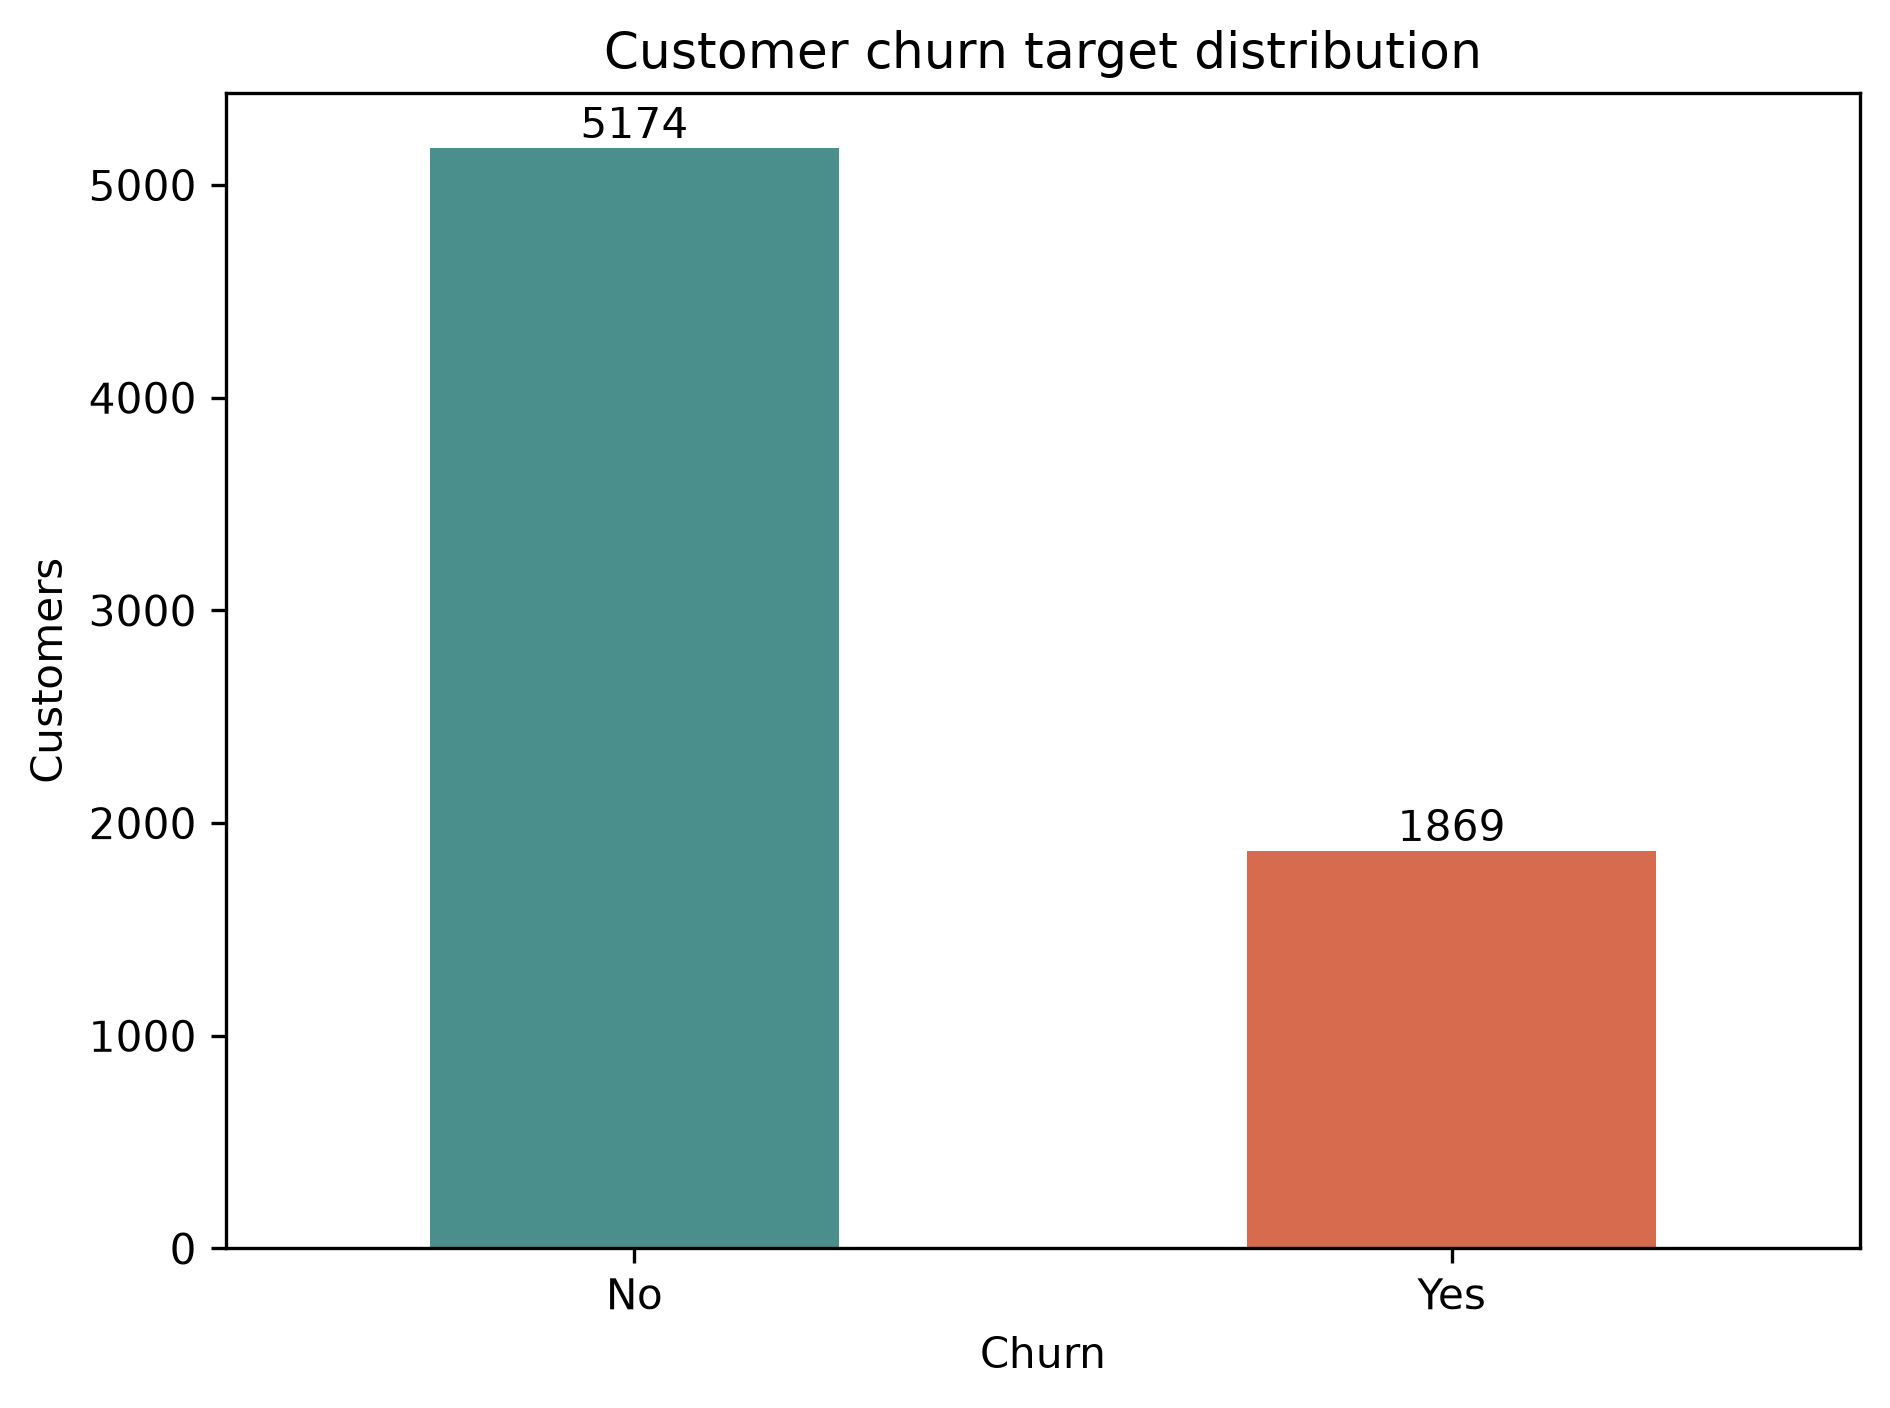
\includegraphics[width=0.75\textwidth]{../graphics/customer_churn_target_distribution.png}
\caption{\centering Distribution of customers by churn status.}
\label{fig:churn-target-distribution}
\end{figure}



\subsection{Feature Statistics}
Table~\ref{tab:numeric-summary} summarizes the non-binary numeric features: customer tenure and charges. The binary \texttt{SeniorCitizen} feature is excluded from these measurements.

\begin{table}[H]
\centering
\small
\begin{tabular}{lrrrrr}
\toprule
\textbf{Feature} & \textbf{N} & \textbf{Mean} & \textbf{SD} & \textbf{Min} & \textbf{Max} \\
\midrule
tenure (months) & 7,043 & 32.37 & 24.56 & 0 & 72 \\
MonthlyCharges & 7,043 & 64.76 & 30.09 & 18.25 & 118.75 \\
TotalCharges & 7,032 & 2,283.30 & 2,266.77 & 18.80 & 8,684.80 \\
\bottomrule
\end{tabular}
\caption{\centering Summary statistics for numeric features.}
\label{tab:numeric-summary}
\end{table}

\begin{figure}[H]
\centering
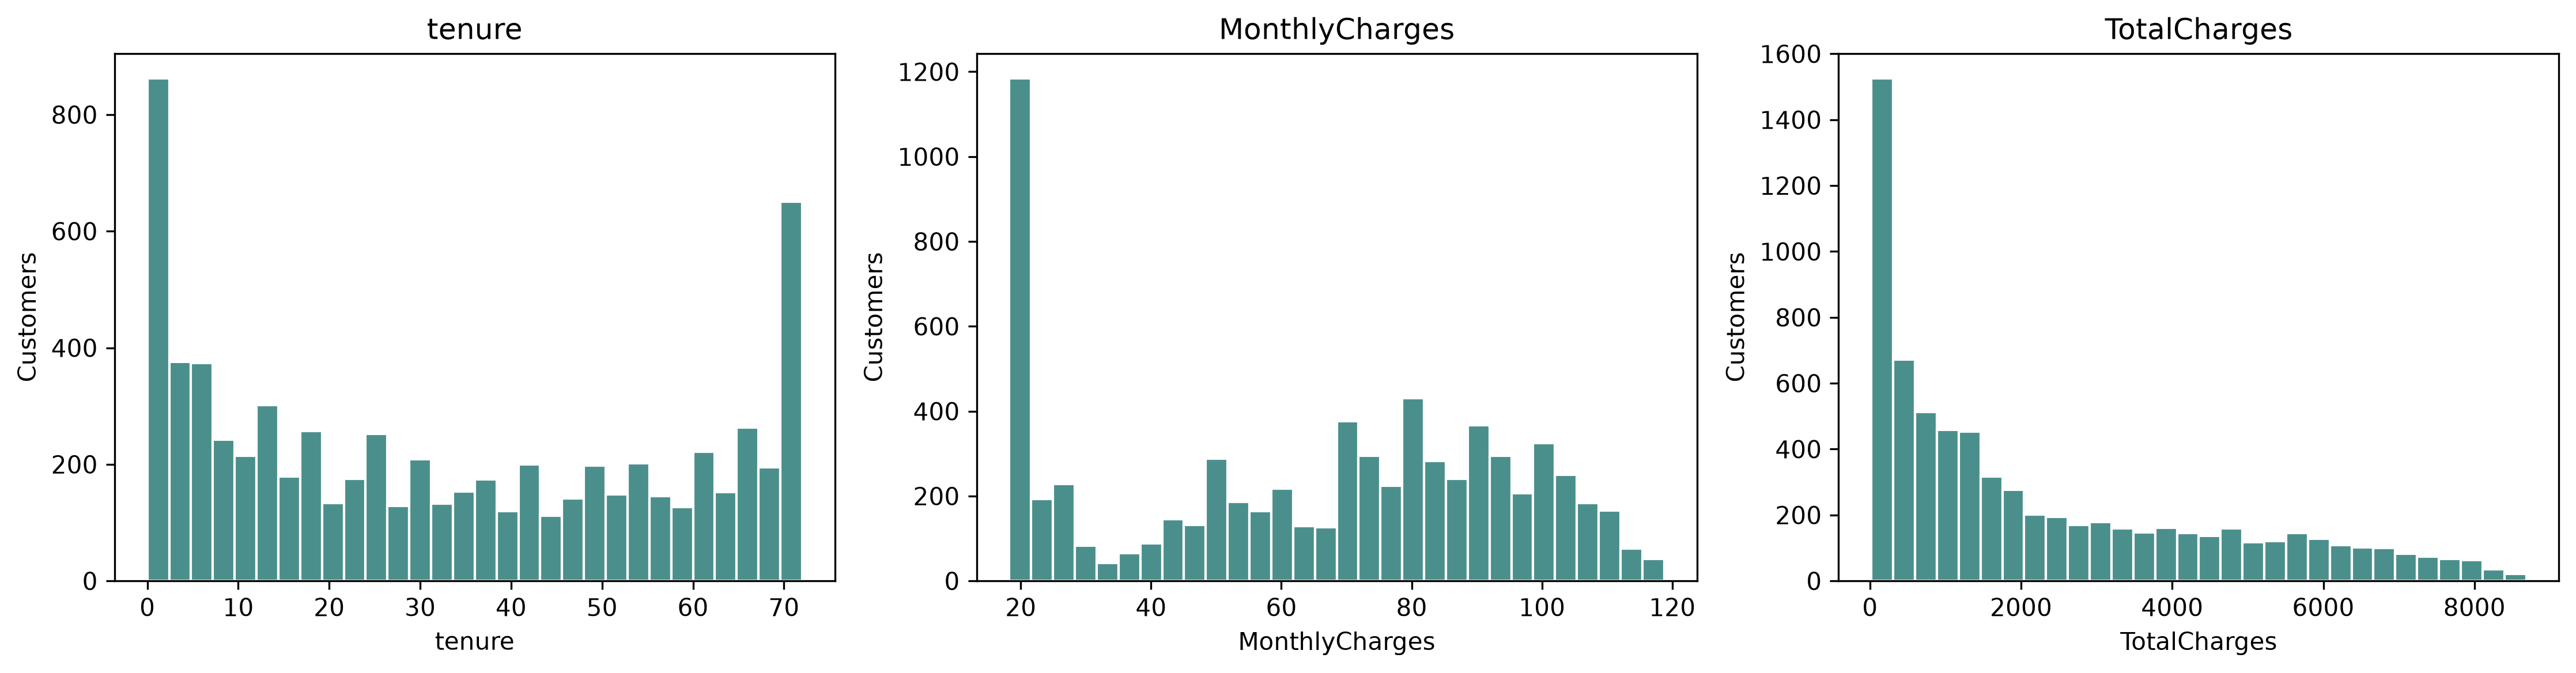
\includegraphics[width=0.95\textwidth]{../graphics/numeric_feature_histograms.png}
\caption{\centering Histograms of tenure, monthly charges, and total charges.}
\label{fig:numeric-feature-histograms}
\end{figure}

\subsection{Categorical Features}
The categorical features describe customer demographics and household status, phone and internet services, service add-ons, streaming, contract and billing arrangements, and payment method. Each bar shows the percentage of all 7,043 customers in that category. The unique identifier \texttt{customerID} and target \texttt{Churn} are excluded here; the target distribution is shown separately in Figure~\ref{fig:churn-target-distribution}.

\begin{figure}[H]
\centering
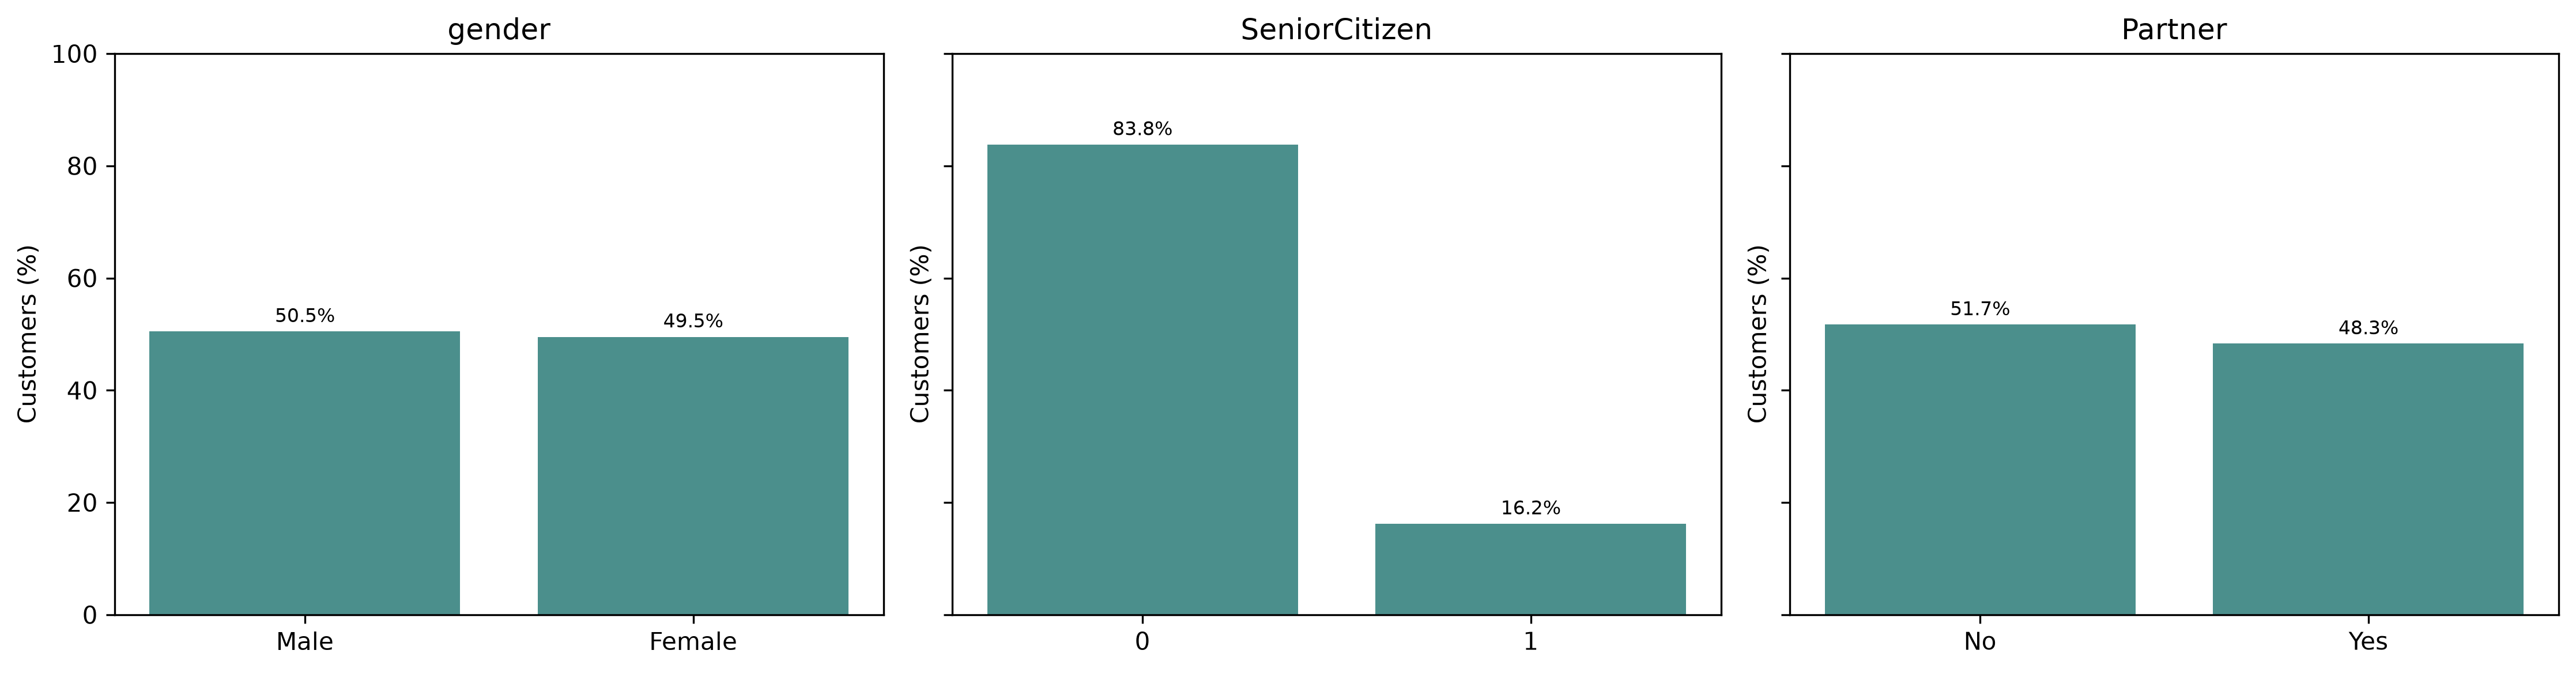
\includegraphics[width=0.95\textwidth]{../graphics/categorical_distributions_01_customer_profile.png}
\caption{\centering Distributions of customer profile features.}
\label{fig:categorical-customer-profile}
\end{figure}

\begin{figure}[H]
\centering
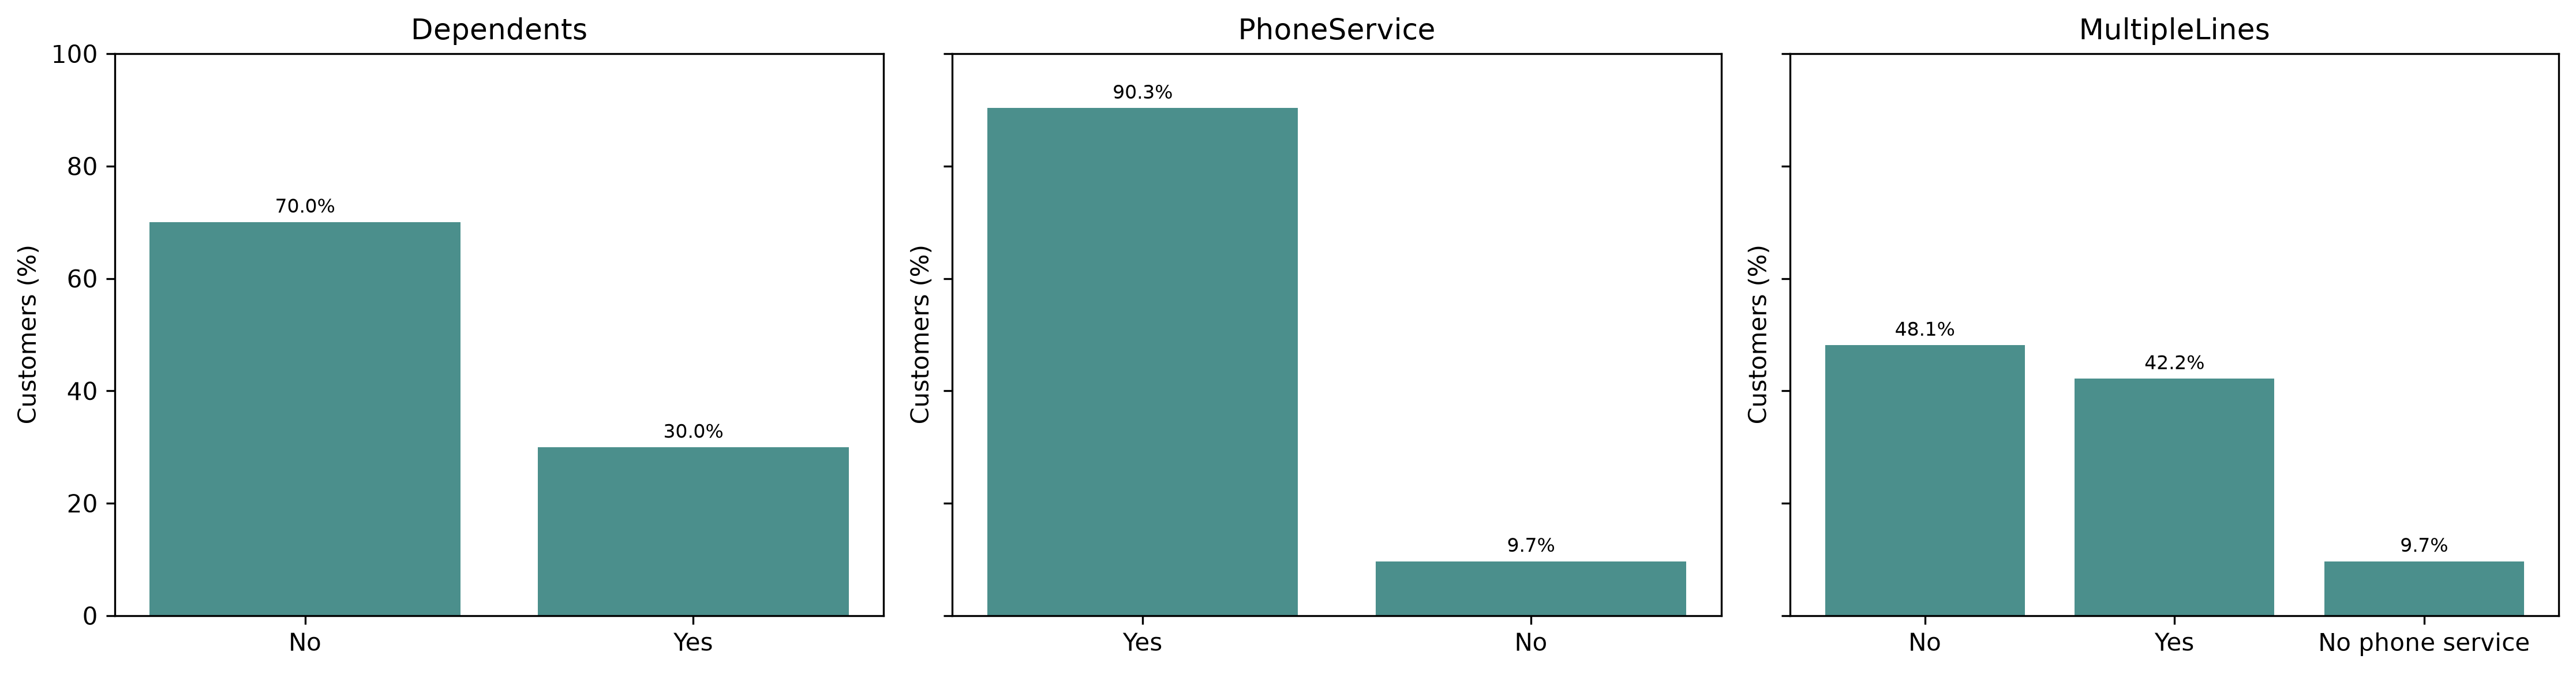
\includegraphics[width=0.95\textwidth]{../graphics/categorical_distributions_02_phone_services.png}
\caption{\centering Distributions of household and phone service features.}
\label{fig:categorical-phone-services}
\end{figure}

\begin{figure}[H]
\centering
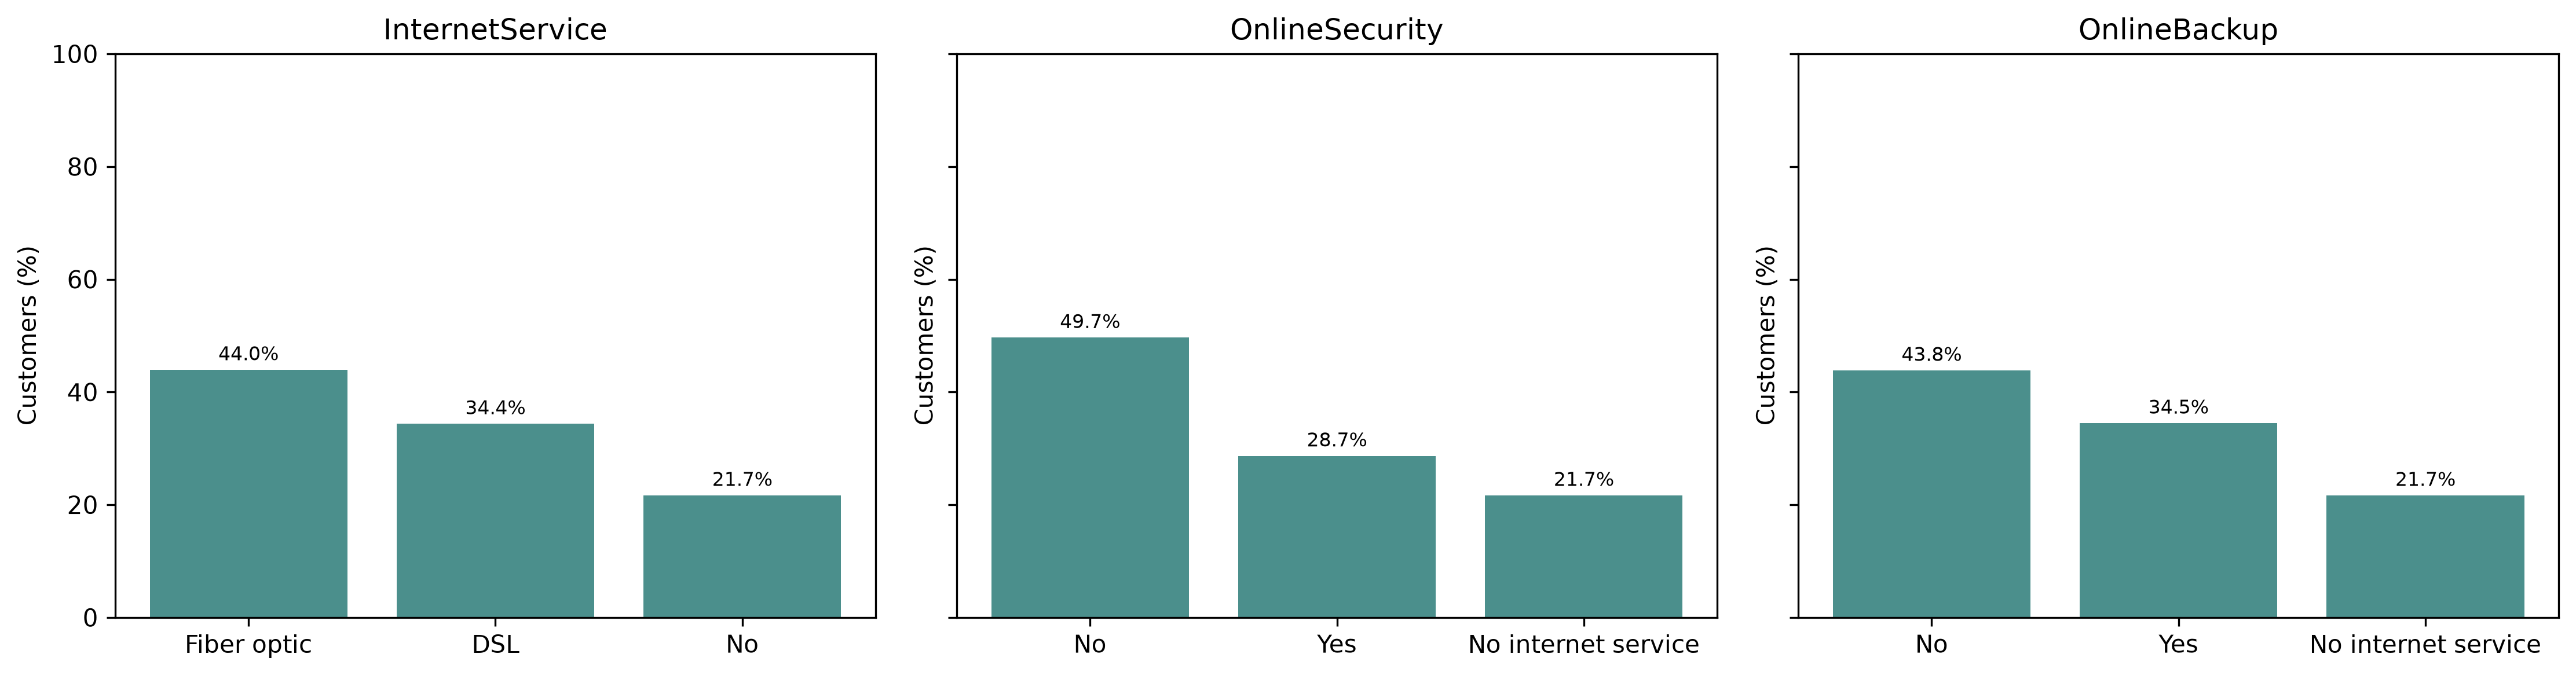
\includegraphics[width=0.95\textwidth]{../graphics/categorical_distributions_03_internet_and_security.png}
\caption{\centering Distributions of internet service and online service features.}
\label{fig:categorical-internet-security}
\end{figure}

\begin{figure}[H]
\centering
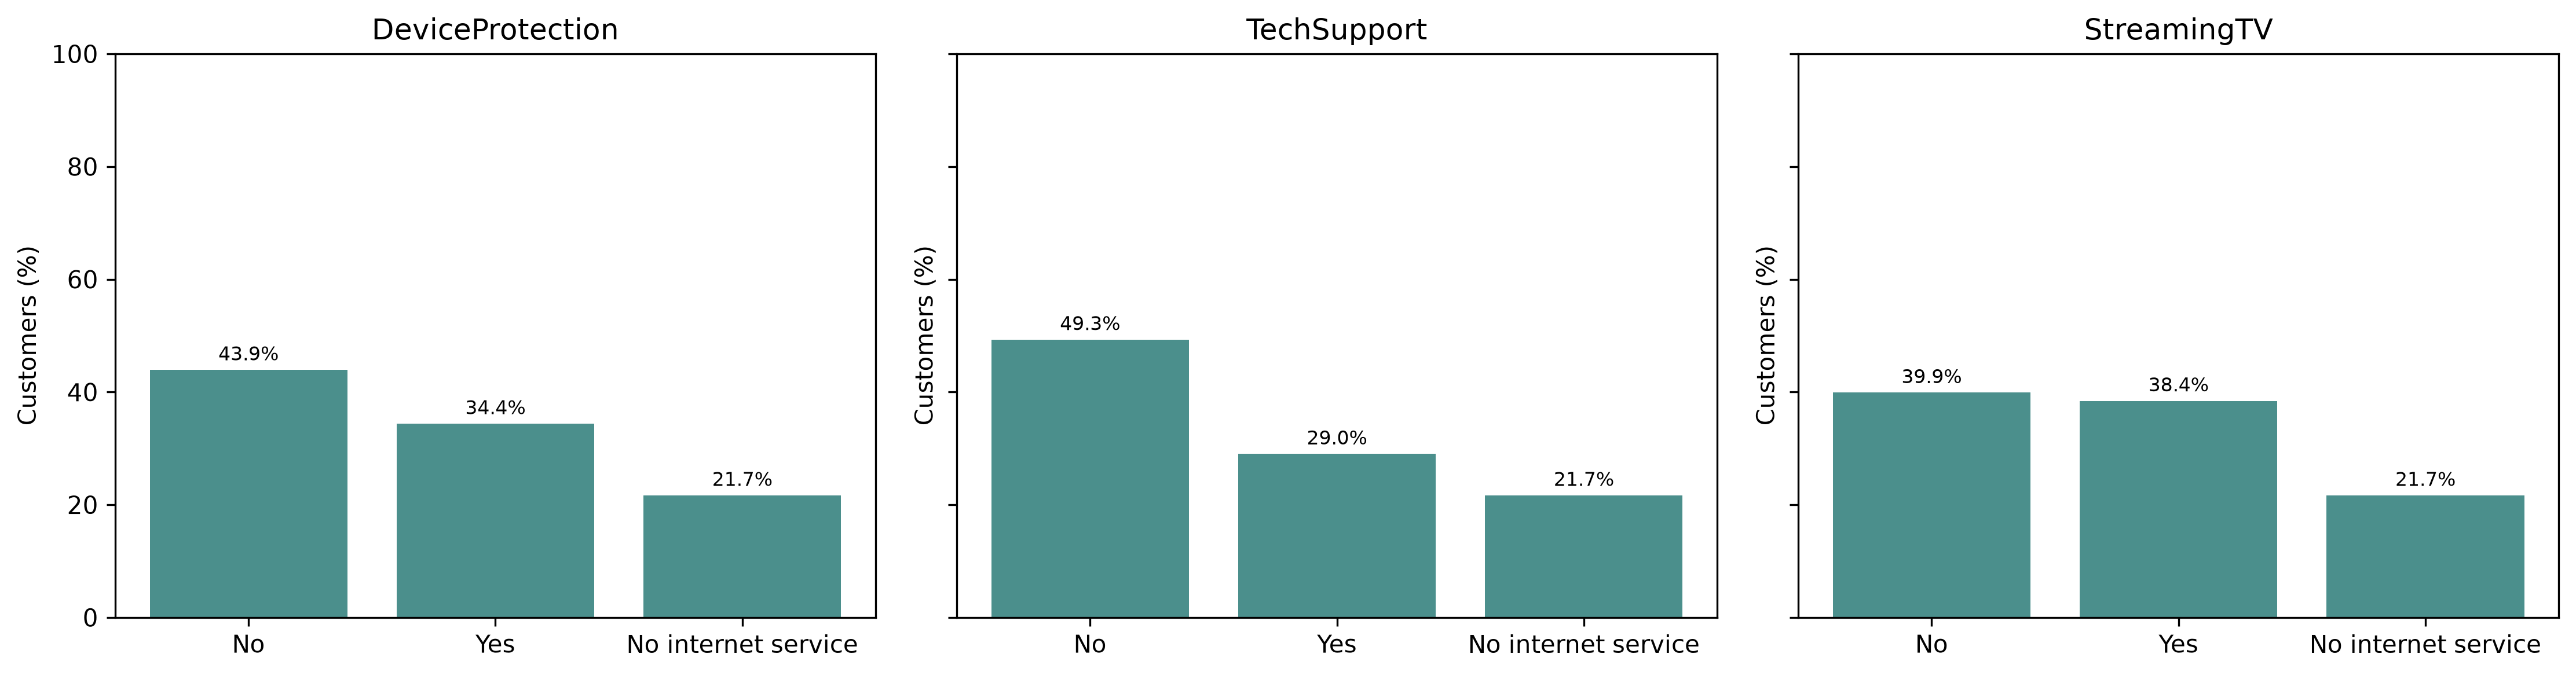
\includegraphics[width=0.95\textwidth]{../graphics/categorical_distributions_04_protection_and_support.png}
\caption{\centering Distributions of device protection, technical support, and streaming TV.}
\label{fig:categorical-protection-support}
\end{figure}

\begin{figure}[H]
\centering
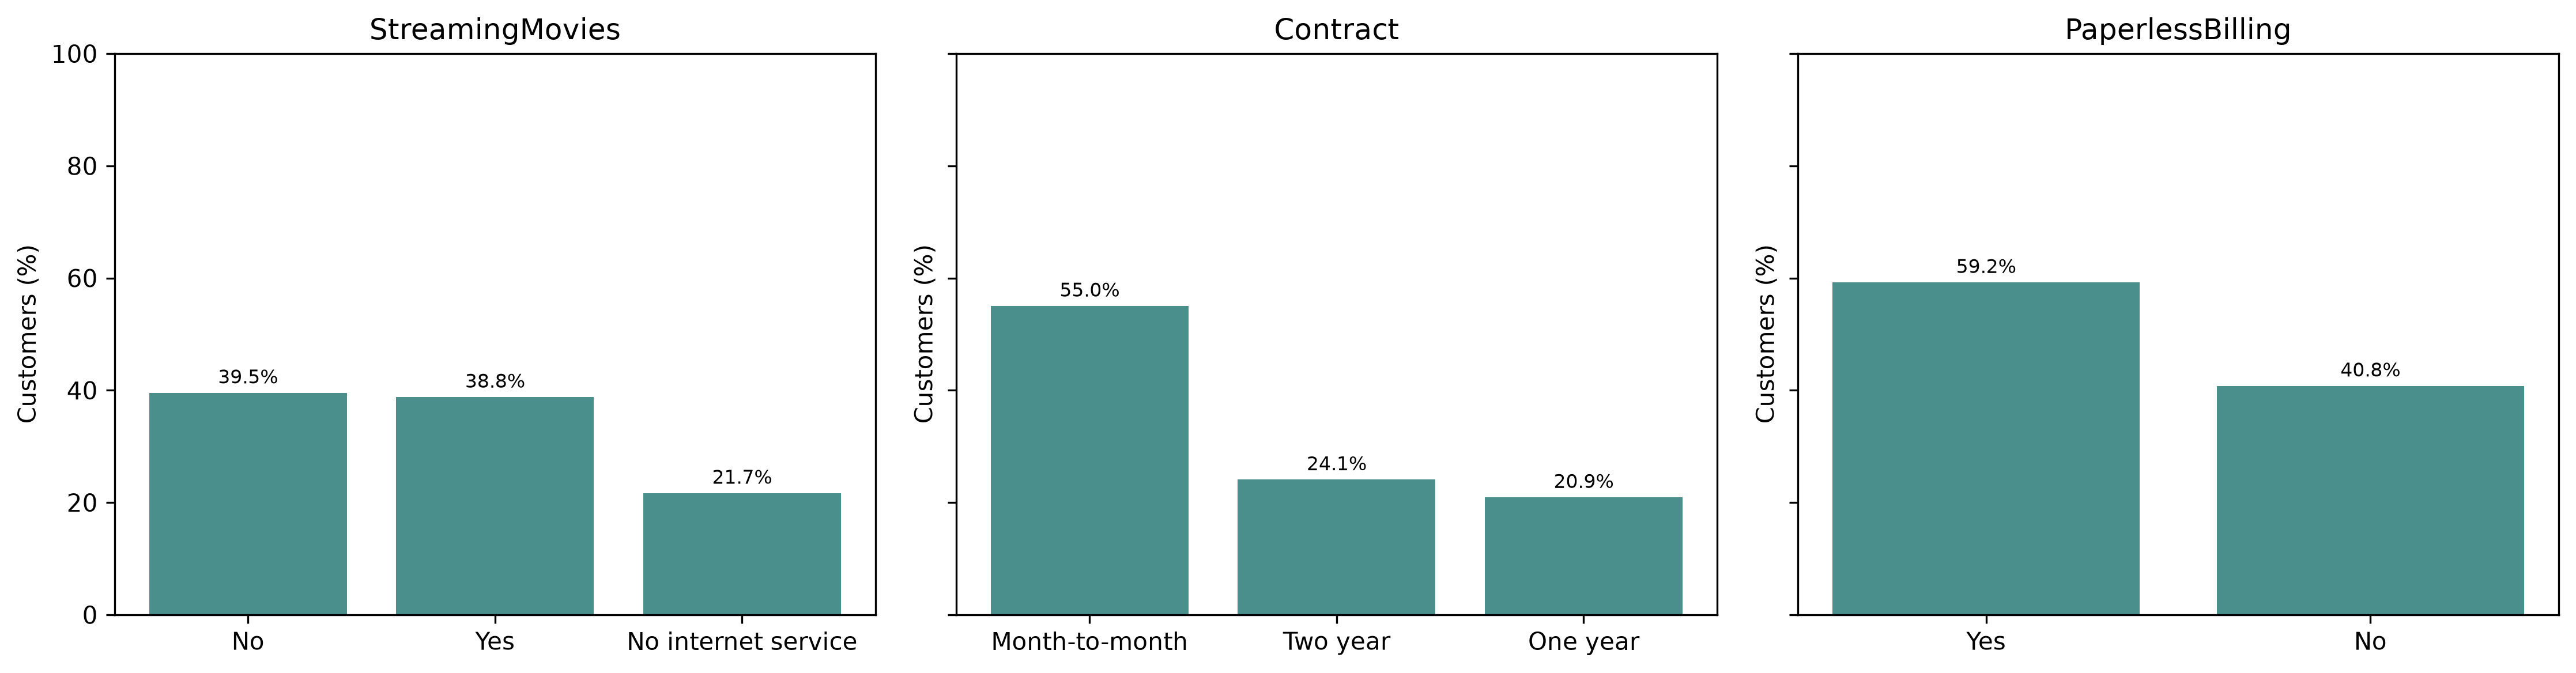
\includegraphics[width=0.95\textwidth]{../graphics/categorical_distributions_05_streaming_and_contract.png}
\caption{\centering Distributions of streaming movies, contract, and paperless billing.}
\label{fig:categorical-streaming-contract}
\end{figure}

\begin{figure}[H]
\centering
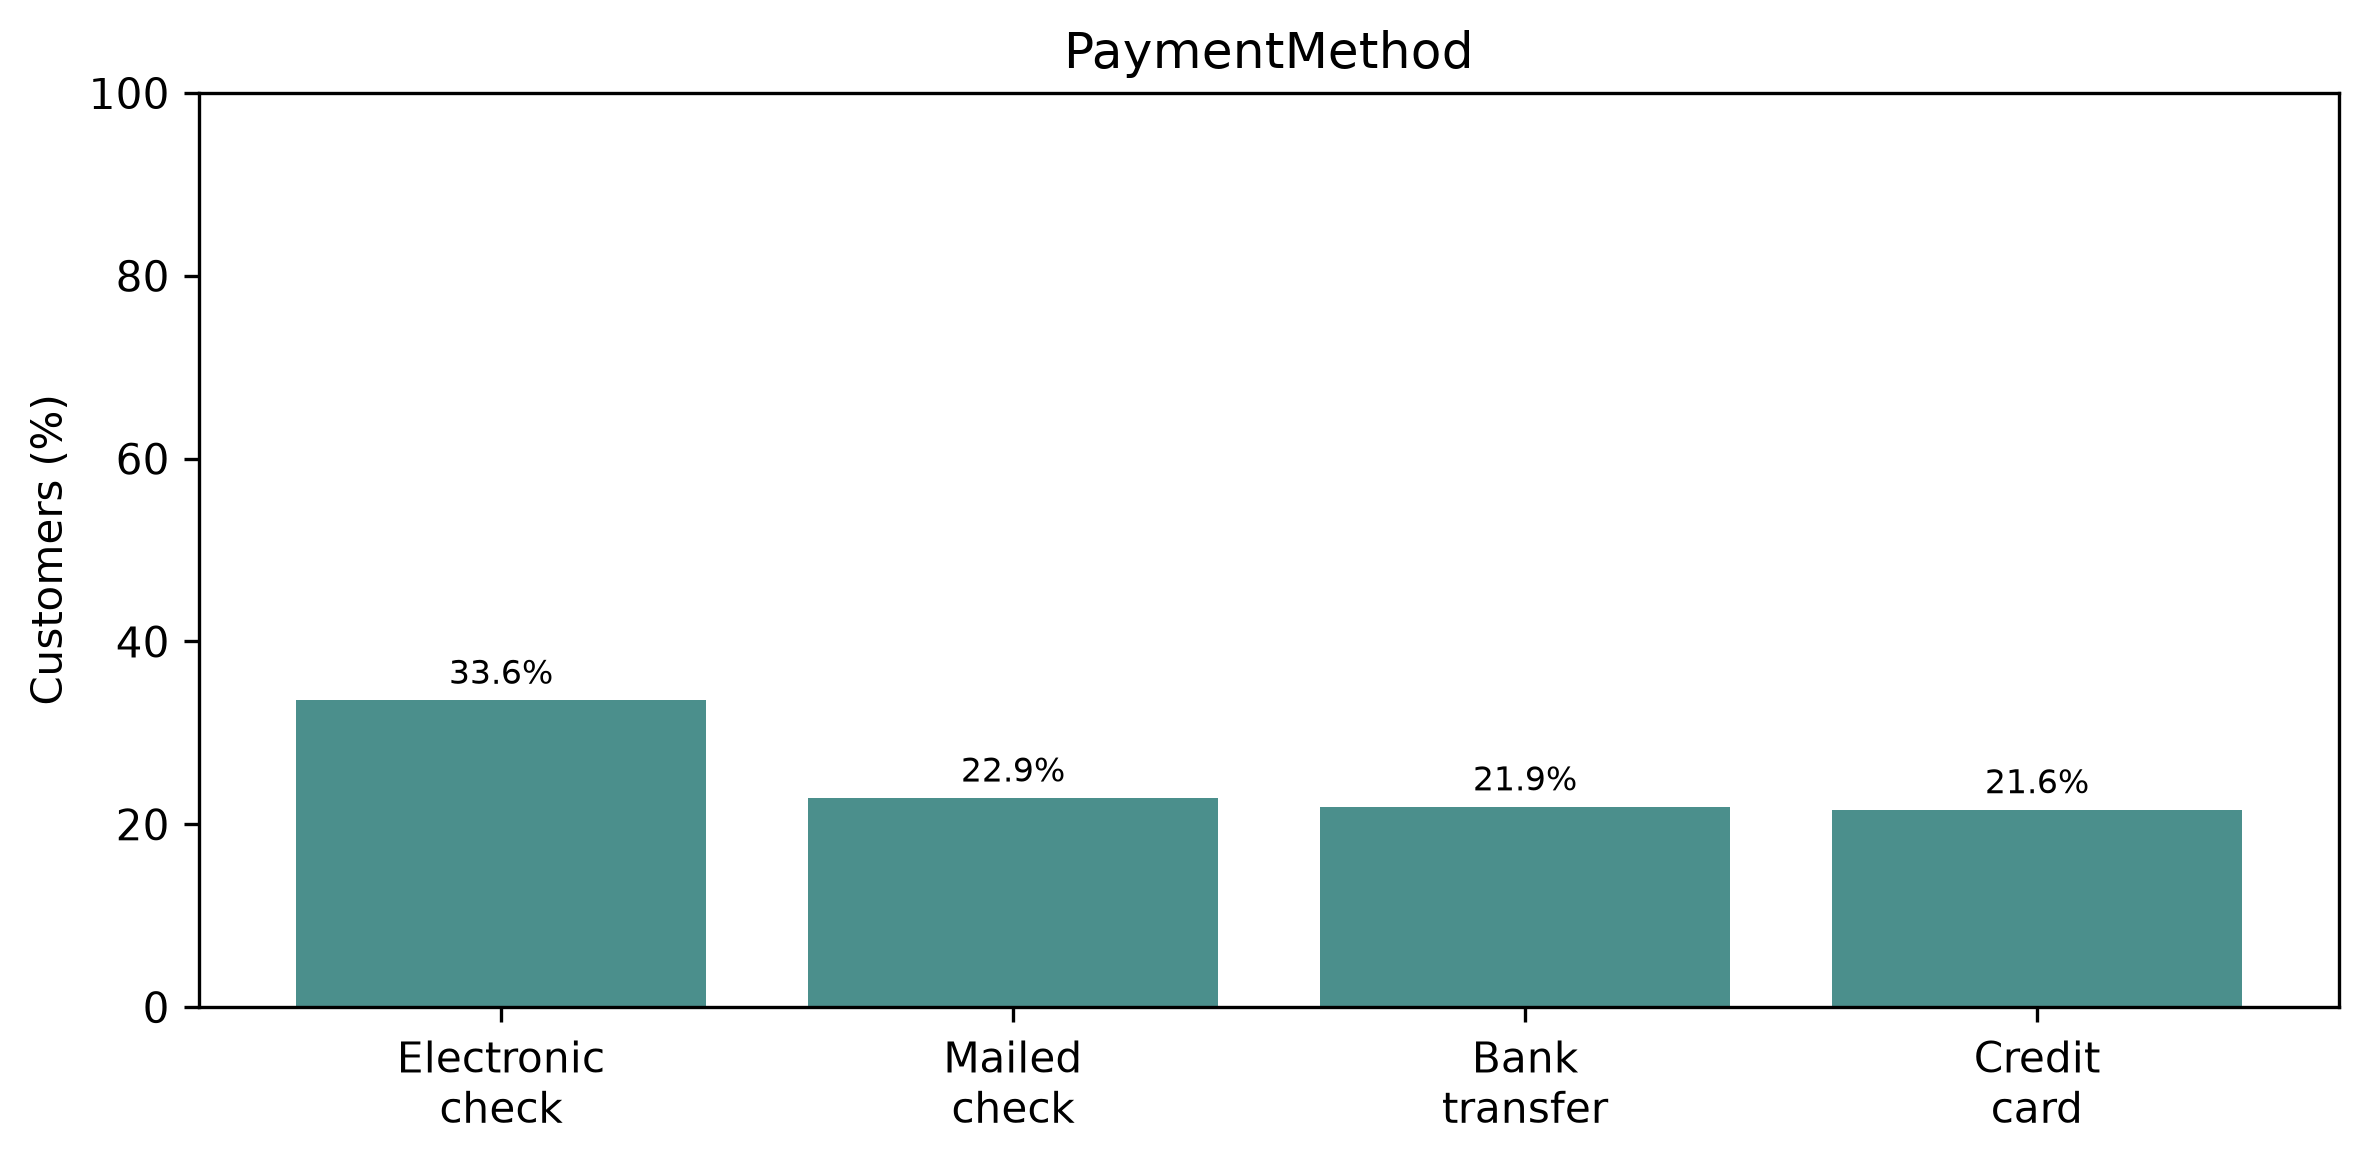
\includegraphics[width=0.95\textwidth]{../graphics/categorical_distributions_06_payment_method.png}
\caption{\centering Distribution of customer payment methods.}
\label{fig:categorical-payment-method}
\end{figure}

\subsection{Data Quality}
The CSV contains no parsed missing cells or duplicate rows, and all 7,043 customer IDs are unique. However, 
11 \texttt{TotalCharges} values are blank strings (0.16\% of records). Is a little portion unusable. There are 7,032 values equal (99.84\% of records ) 

\subsection{Feature Relationships}
These charts compare each feature with the churn target to identify differences between customers who stayed and those who left. The numerical-feature boxplots compare the distributions of tenure, monthly charges, and total charges across the two target classes. For categorical features, each pair of bars shows the percentage of customers within a category who stayed or churned; the two percentages sum to 100\% for each category. These are descriptive associations and do not establish causation.

The numerical comparisons show that churned customers have a shorter median tenure (10 months versus 38) and higher mean monthly charges (74.44 versus 61.27). Among categorical features, churn is more common for month-to-month contracts (42.7\%) than one-year (11.3\%) or two-year contracts (2.8\%), and for fiber-optic internet (41.9\%) and electronic-check payments (45.3\%).

\begin{figure}[H]
\centering
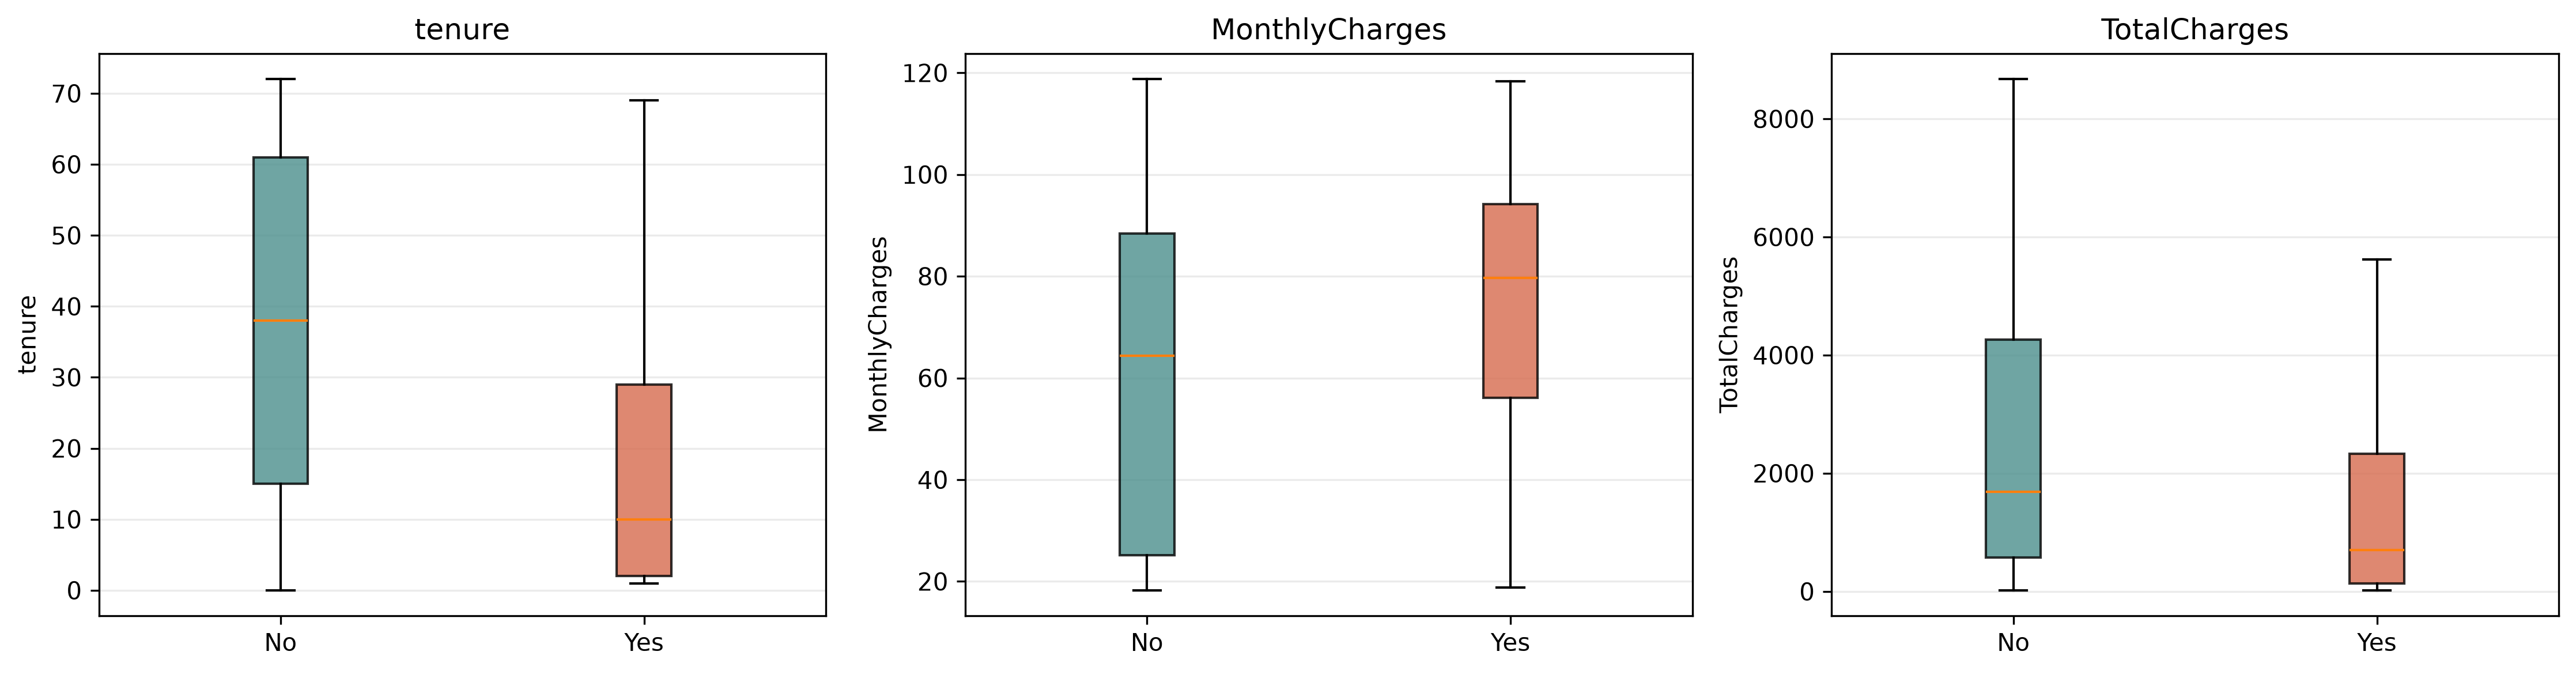
\includegraphics[width=0.95\textwidth]{../graphics/churn_numeric_feature_relationships.png}
\caption{\centering Numeric feature distributions by churn status.}
\label{fig:churn-numeric-relationships}
\end{figure}

\begin{figure}[H]
\centering
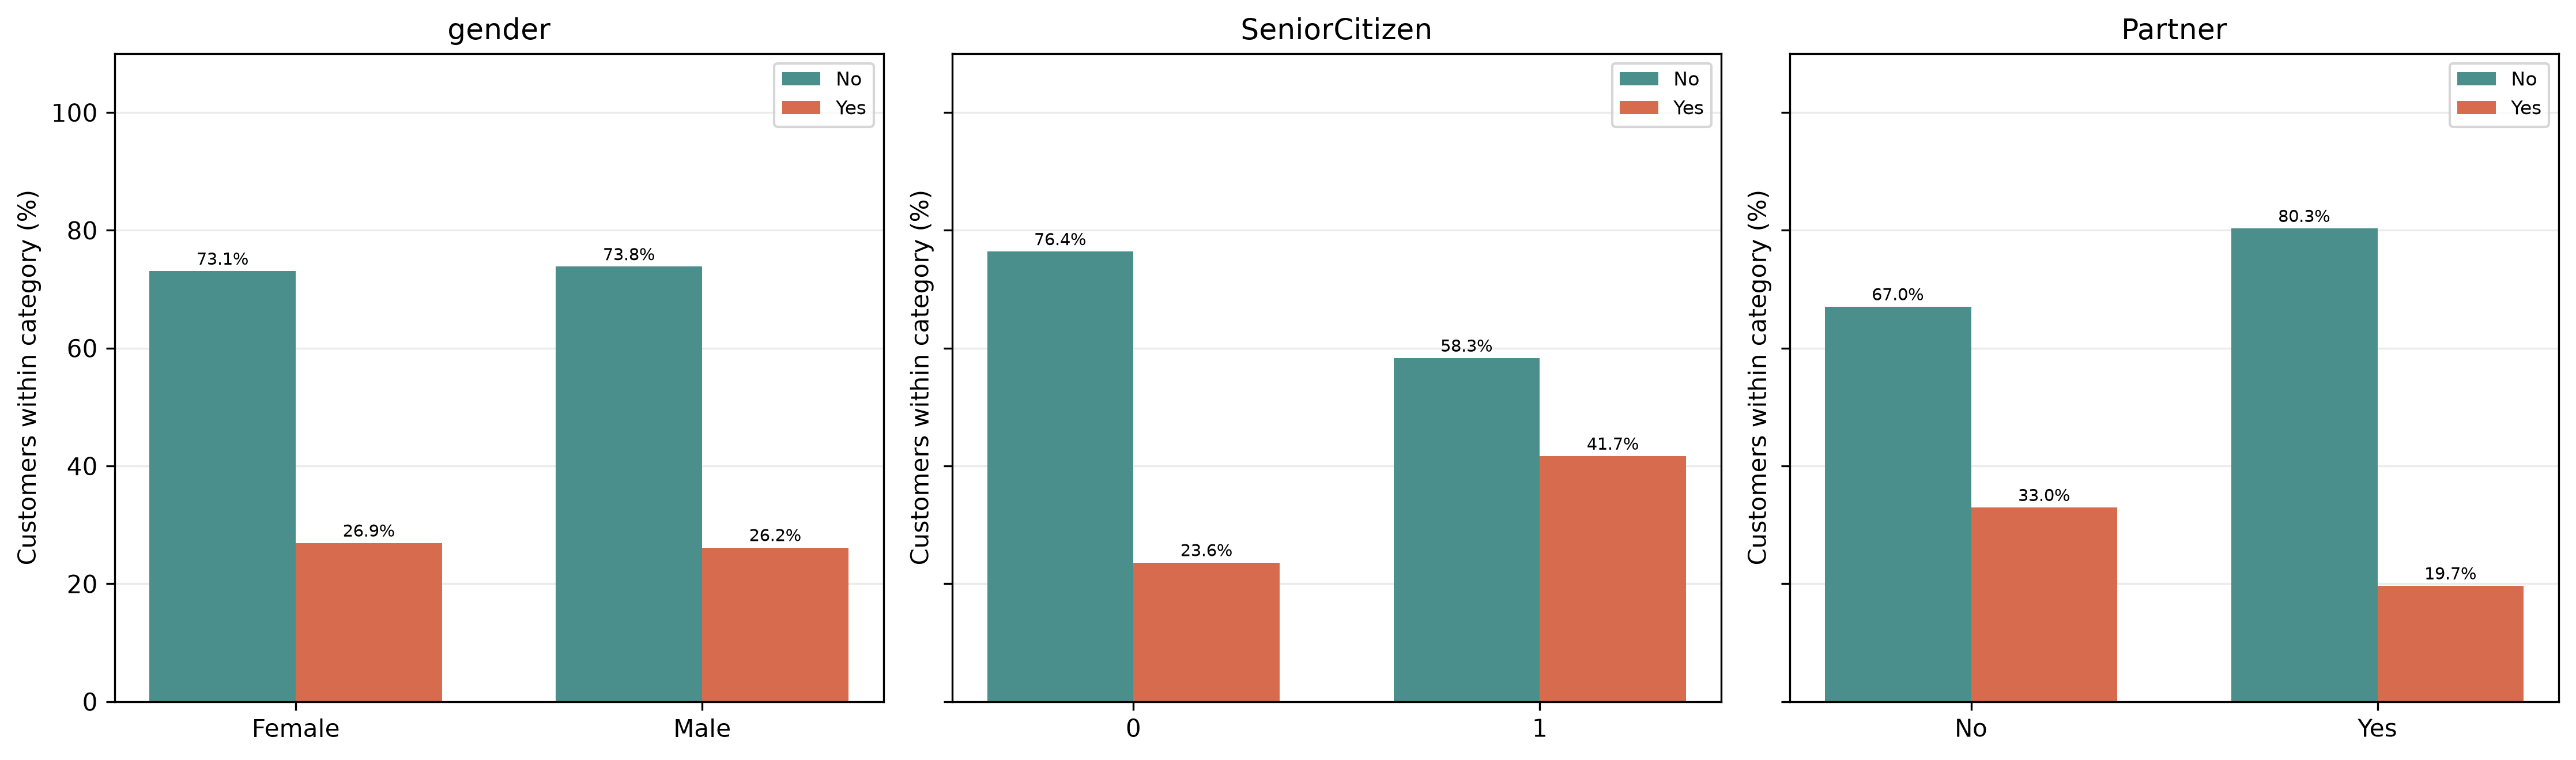
\includegraphics[width=0.95\textwidth]{../graphics/churn_categorical_relationships_01_customer_profile.png}
\caption{\centering Churn rates by customer profile features.}
\label{fig:churn-categorical-profile}
\end{figure}

\begin{figure}[H]
\centering
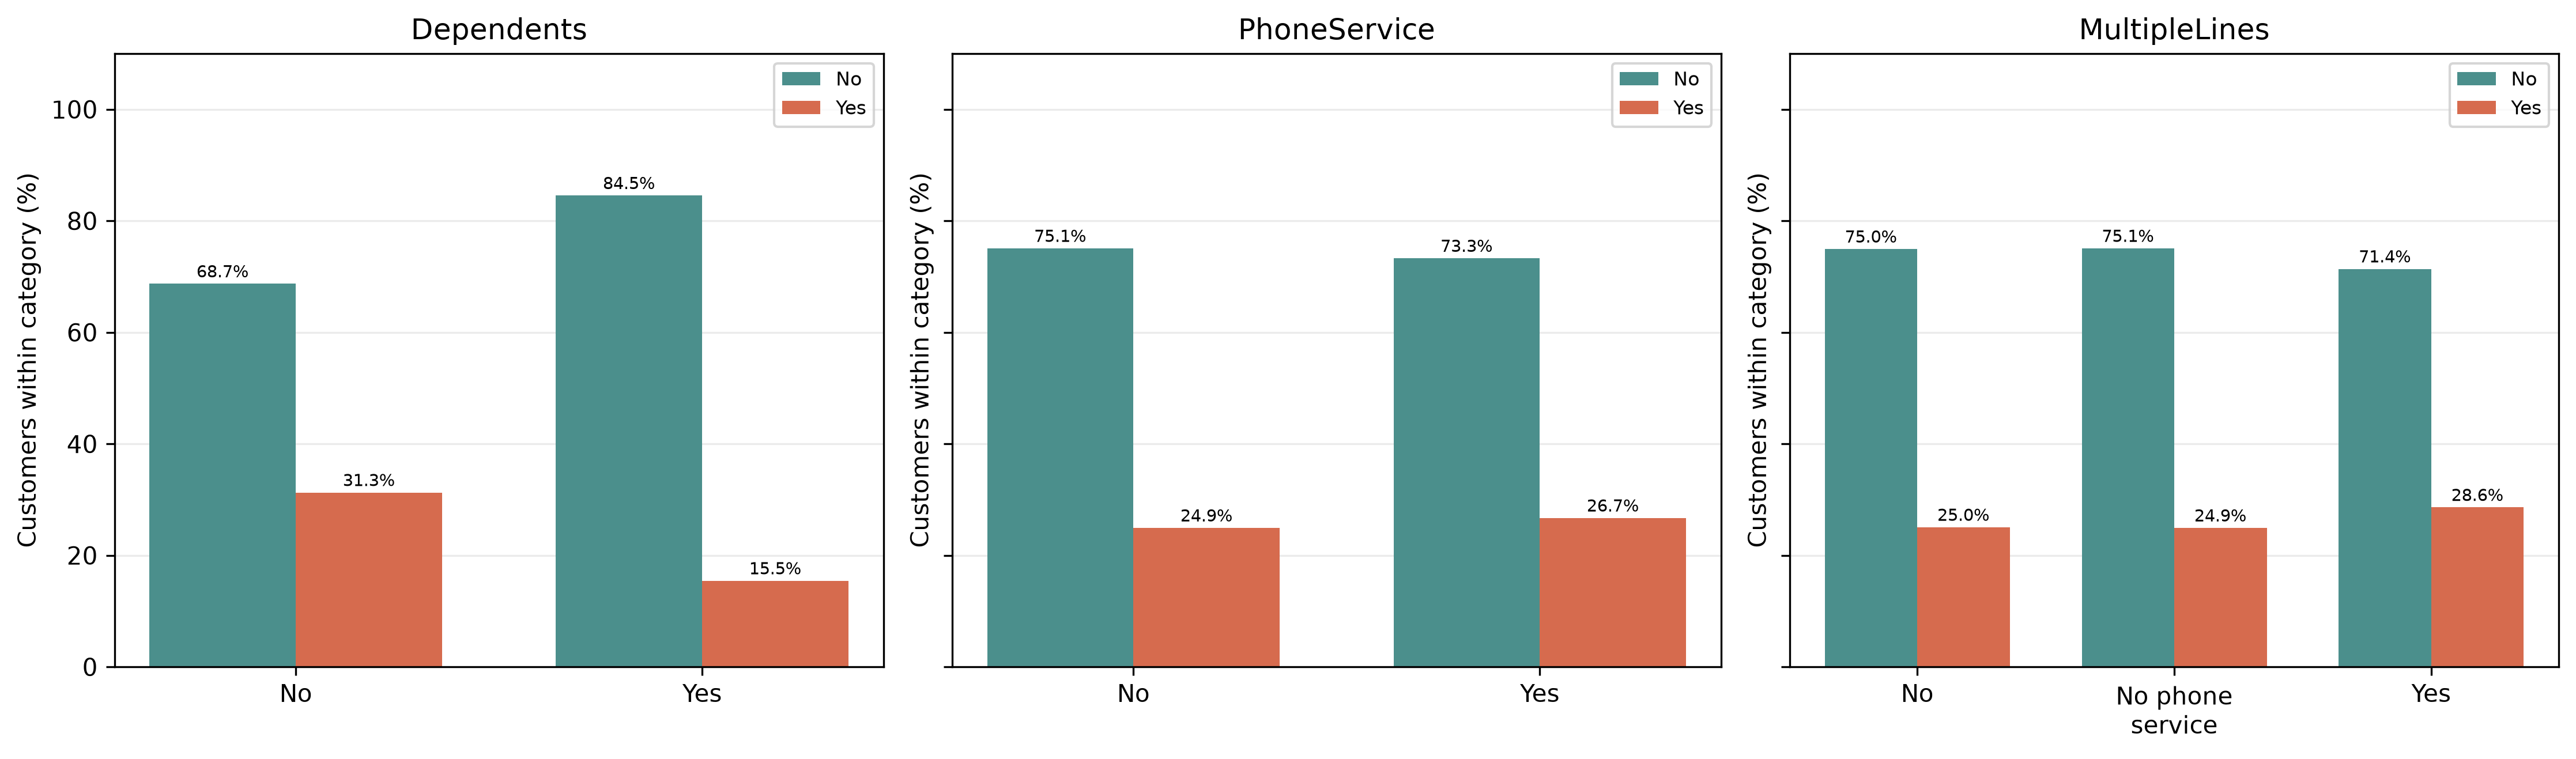
\includegraphics[width=0.95\textwidth]{../graphics/churn_categorical_relationships_02_household_phone.png}
\caption{\centering Churn rates by household and phone features.}
\label{fig:churn-categorical-household-phone}
\end{figure}

\begin{figure}[H]
\centering
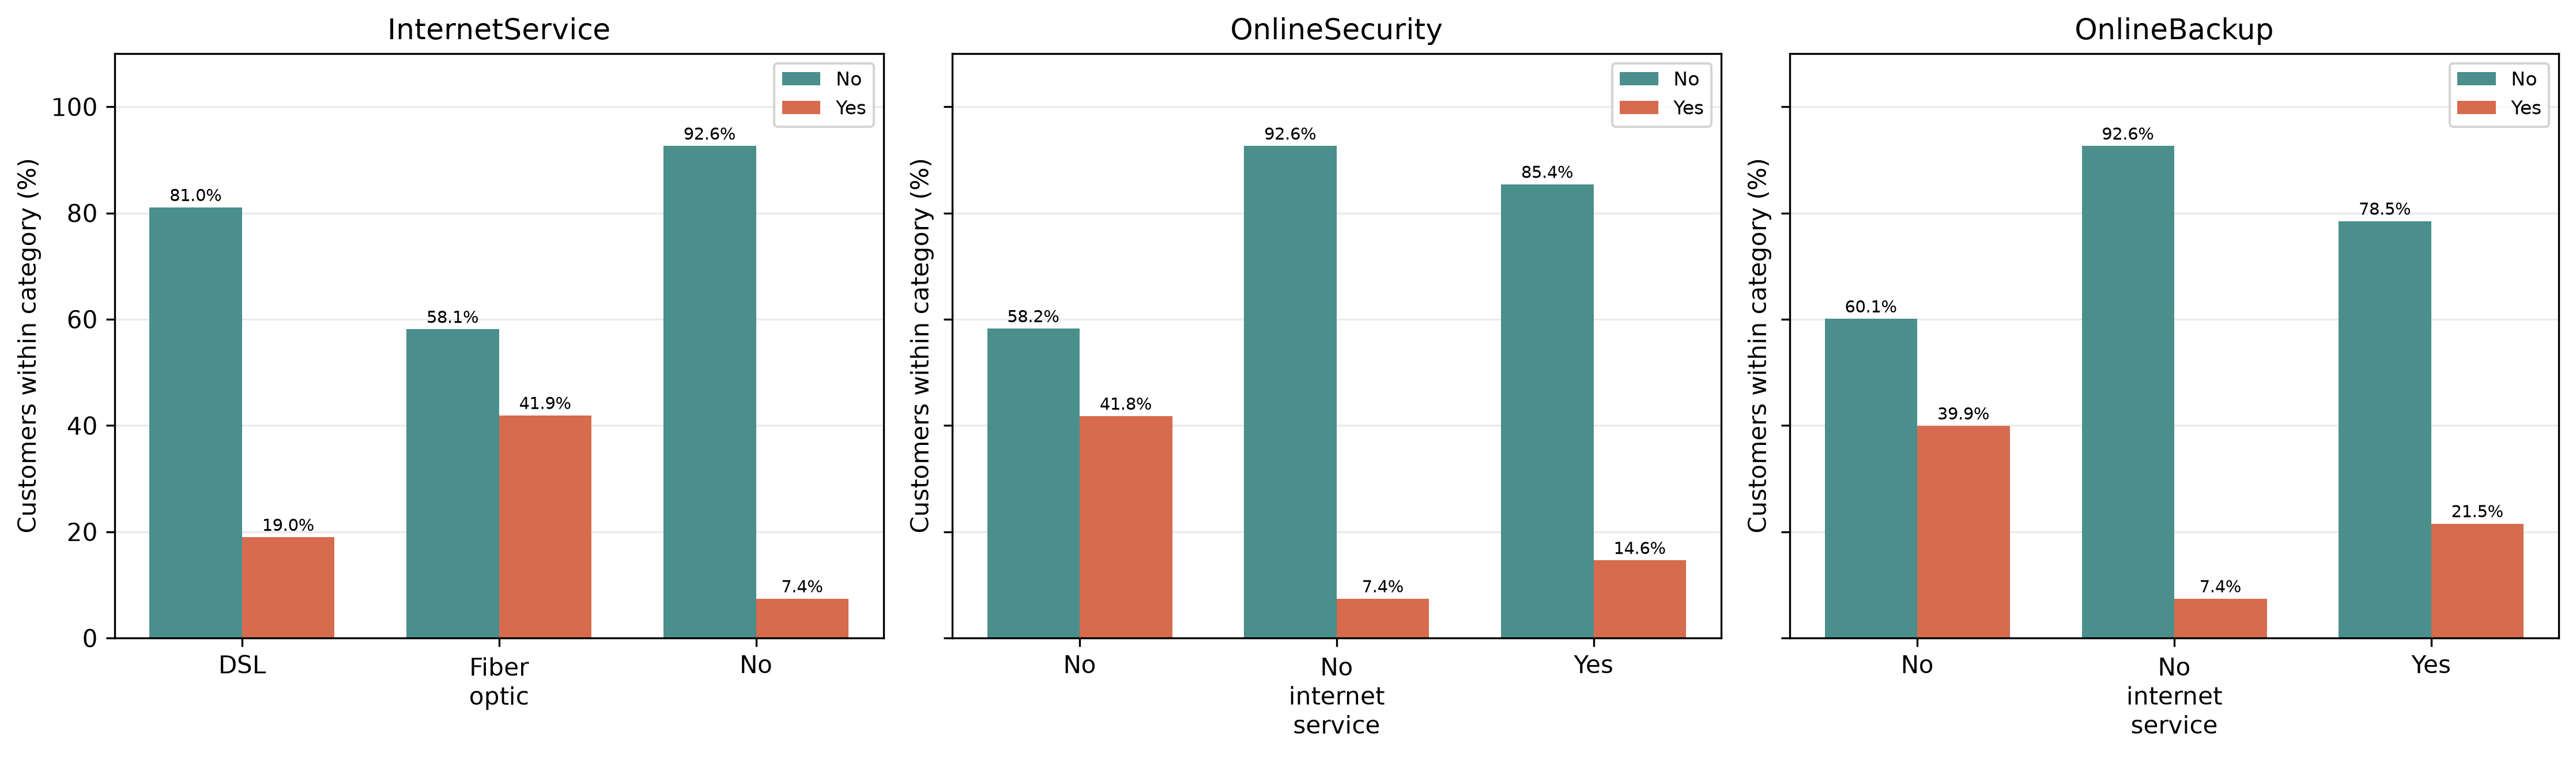
\includegraphics[width=0.95\textwidth]{../graphics/churn_categorical_relationships_03_internet_security.png}
\caption{\centering Churn rates by internet and online security features.}
\label{fig:churn-categorical-internet-security}
\end{figure}

\begin{figure}[H]
\centering
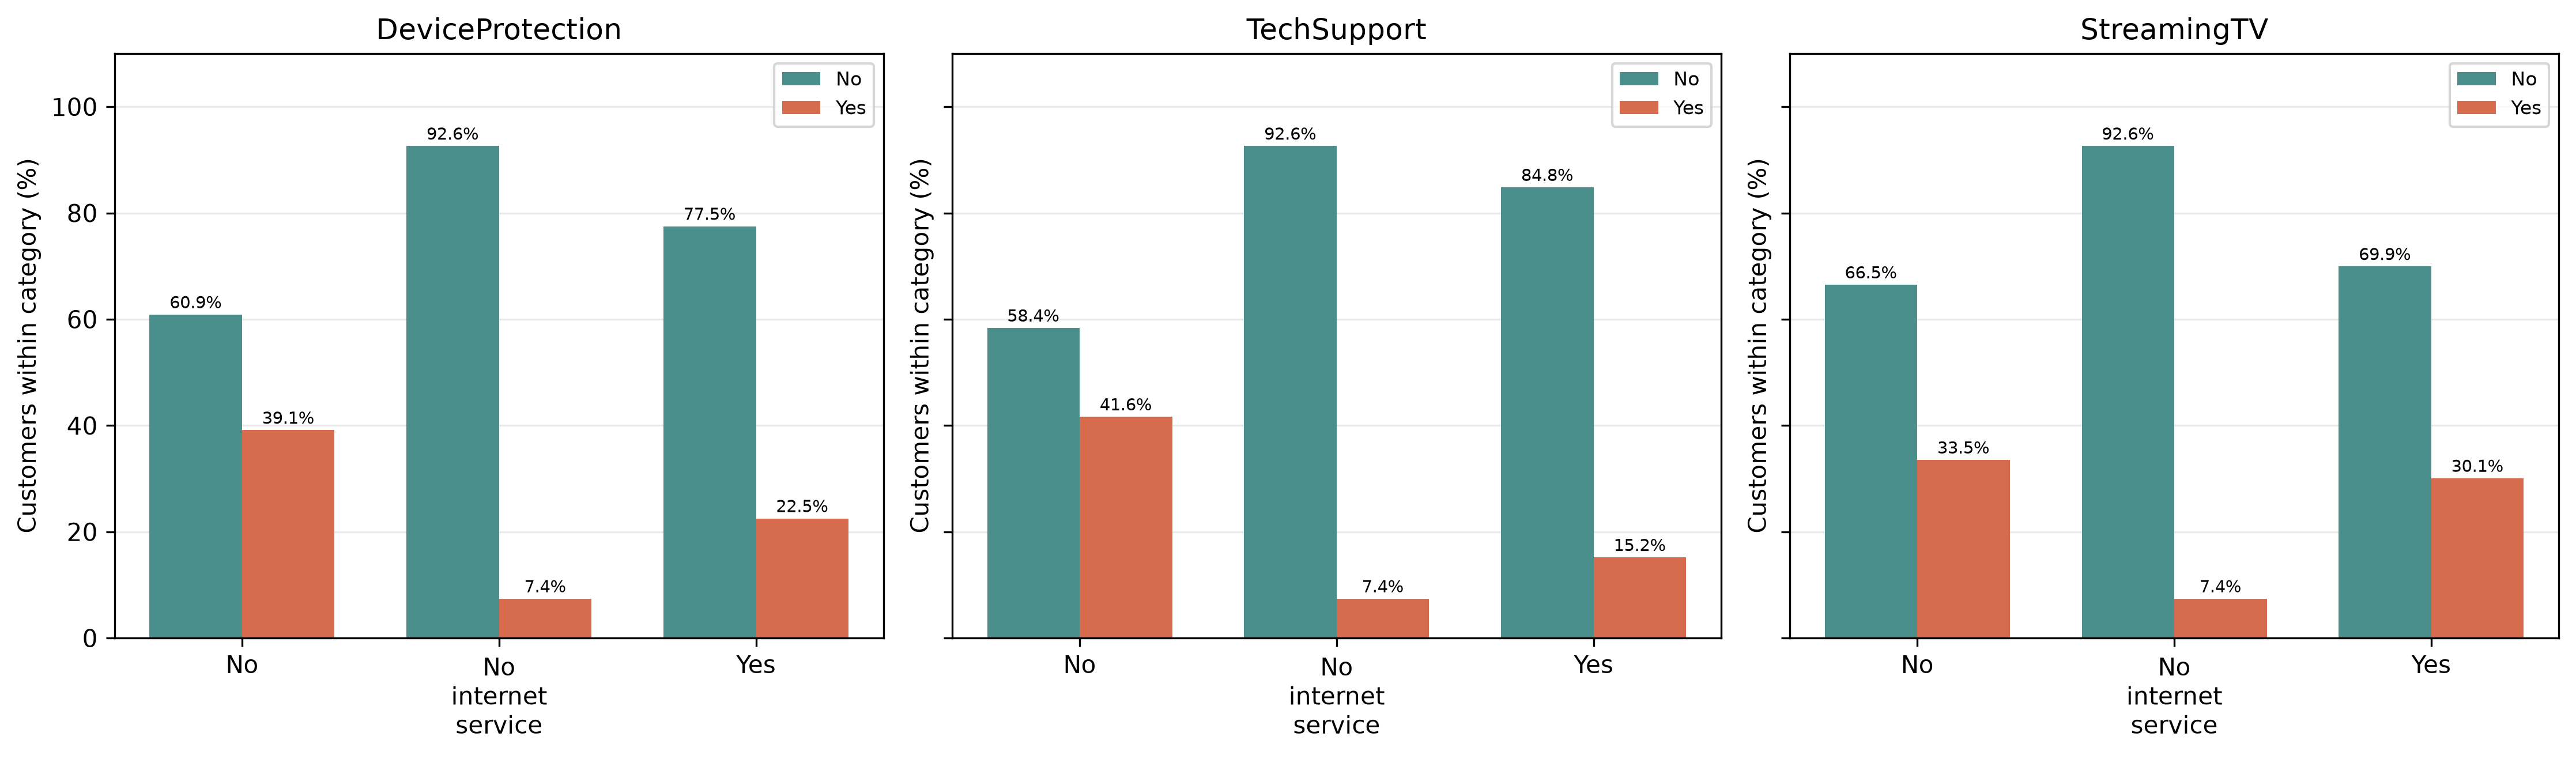
\includegraphics[width=0.95\textwidth]{../graphics/churn_categorical_relationships_04_protection_support.png}
\caption{\centering Churn rates by device protection, tech support, and streaming TV.}
\label{fig:churn-categorical-protection-support}
\end{figure}

\begin{figure}[H]
\centering
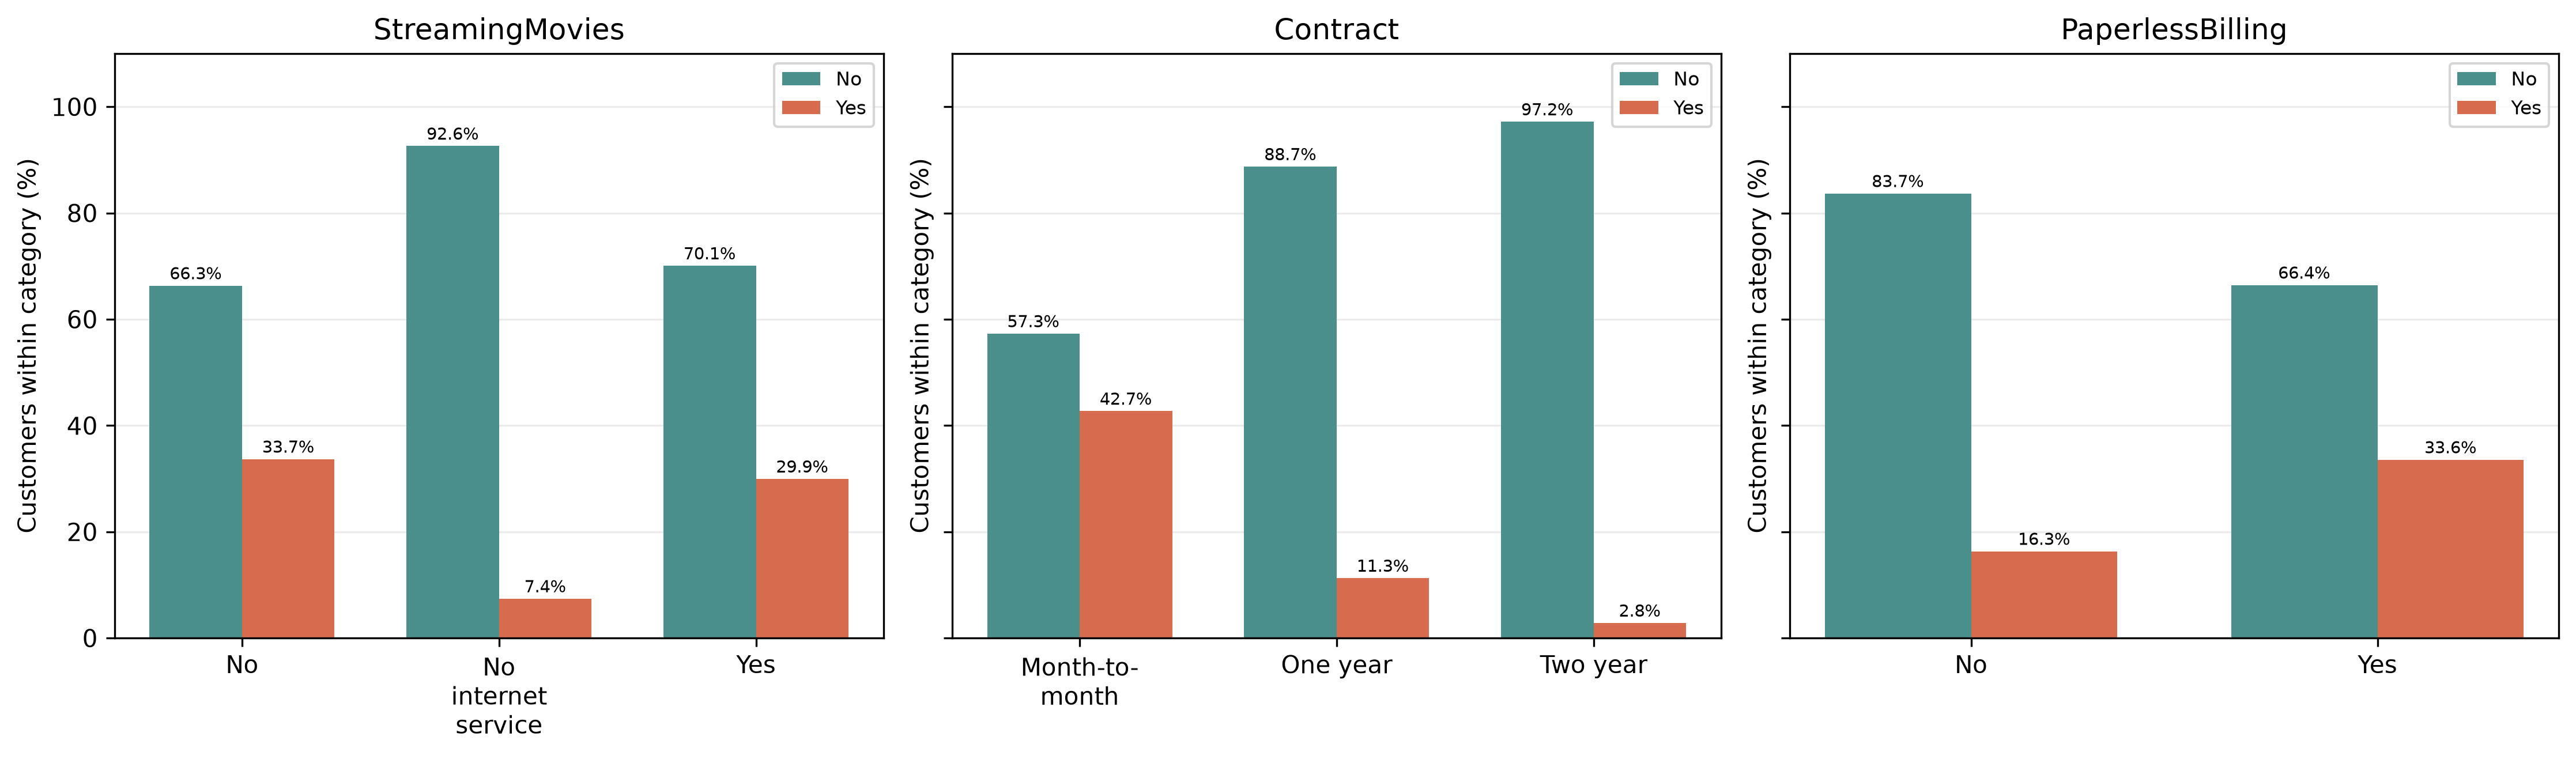
\includegraphics[width=0.95\textwidth]{../graphics/churn_categorical_relationships_05_streaming_contract.png}
\caption{\centering Churn rates by streaming movies, contract, and billing features.}
\label{fig:churn-categorical-streaming-contract}
\end{figure}

\begin{figure}[H]
\centering
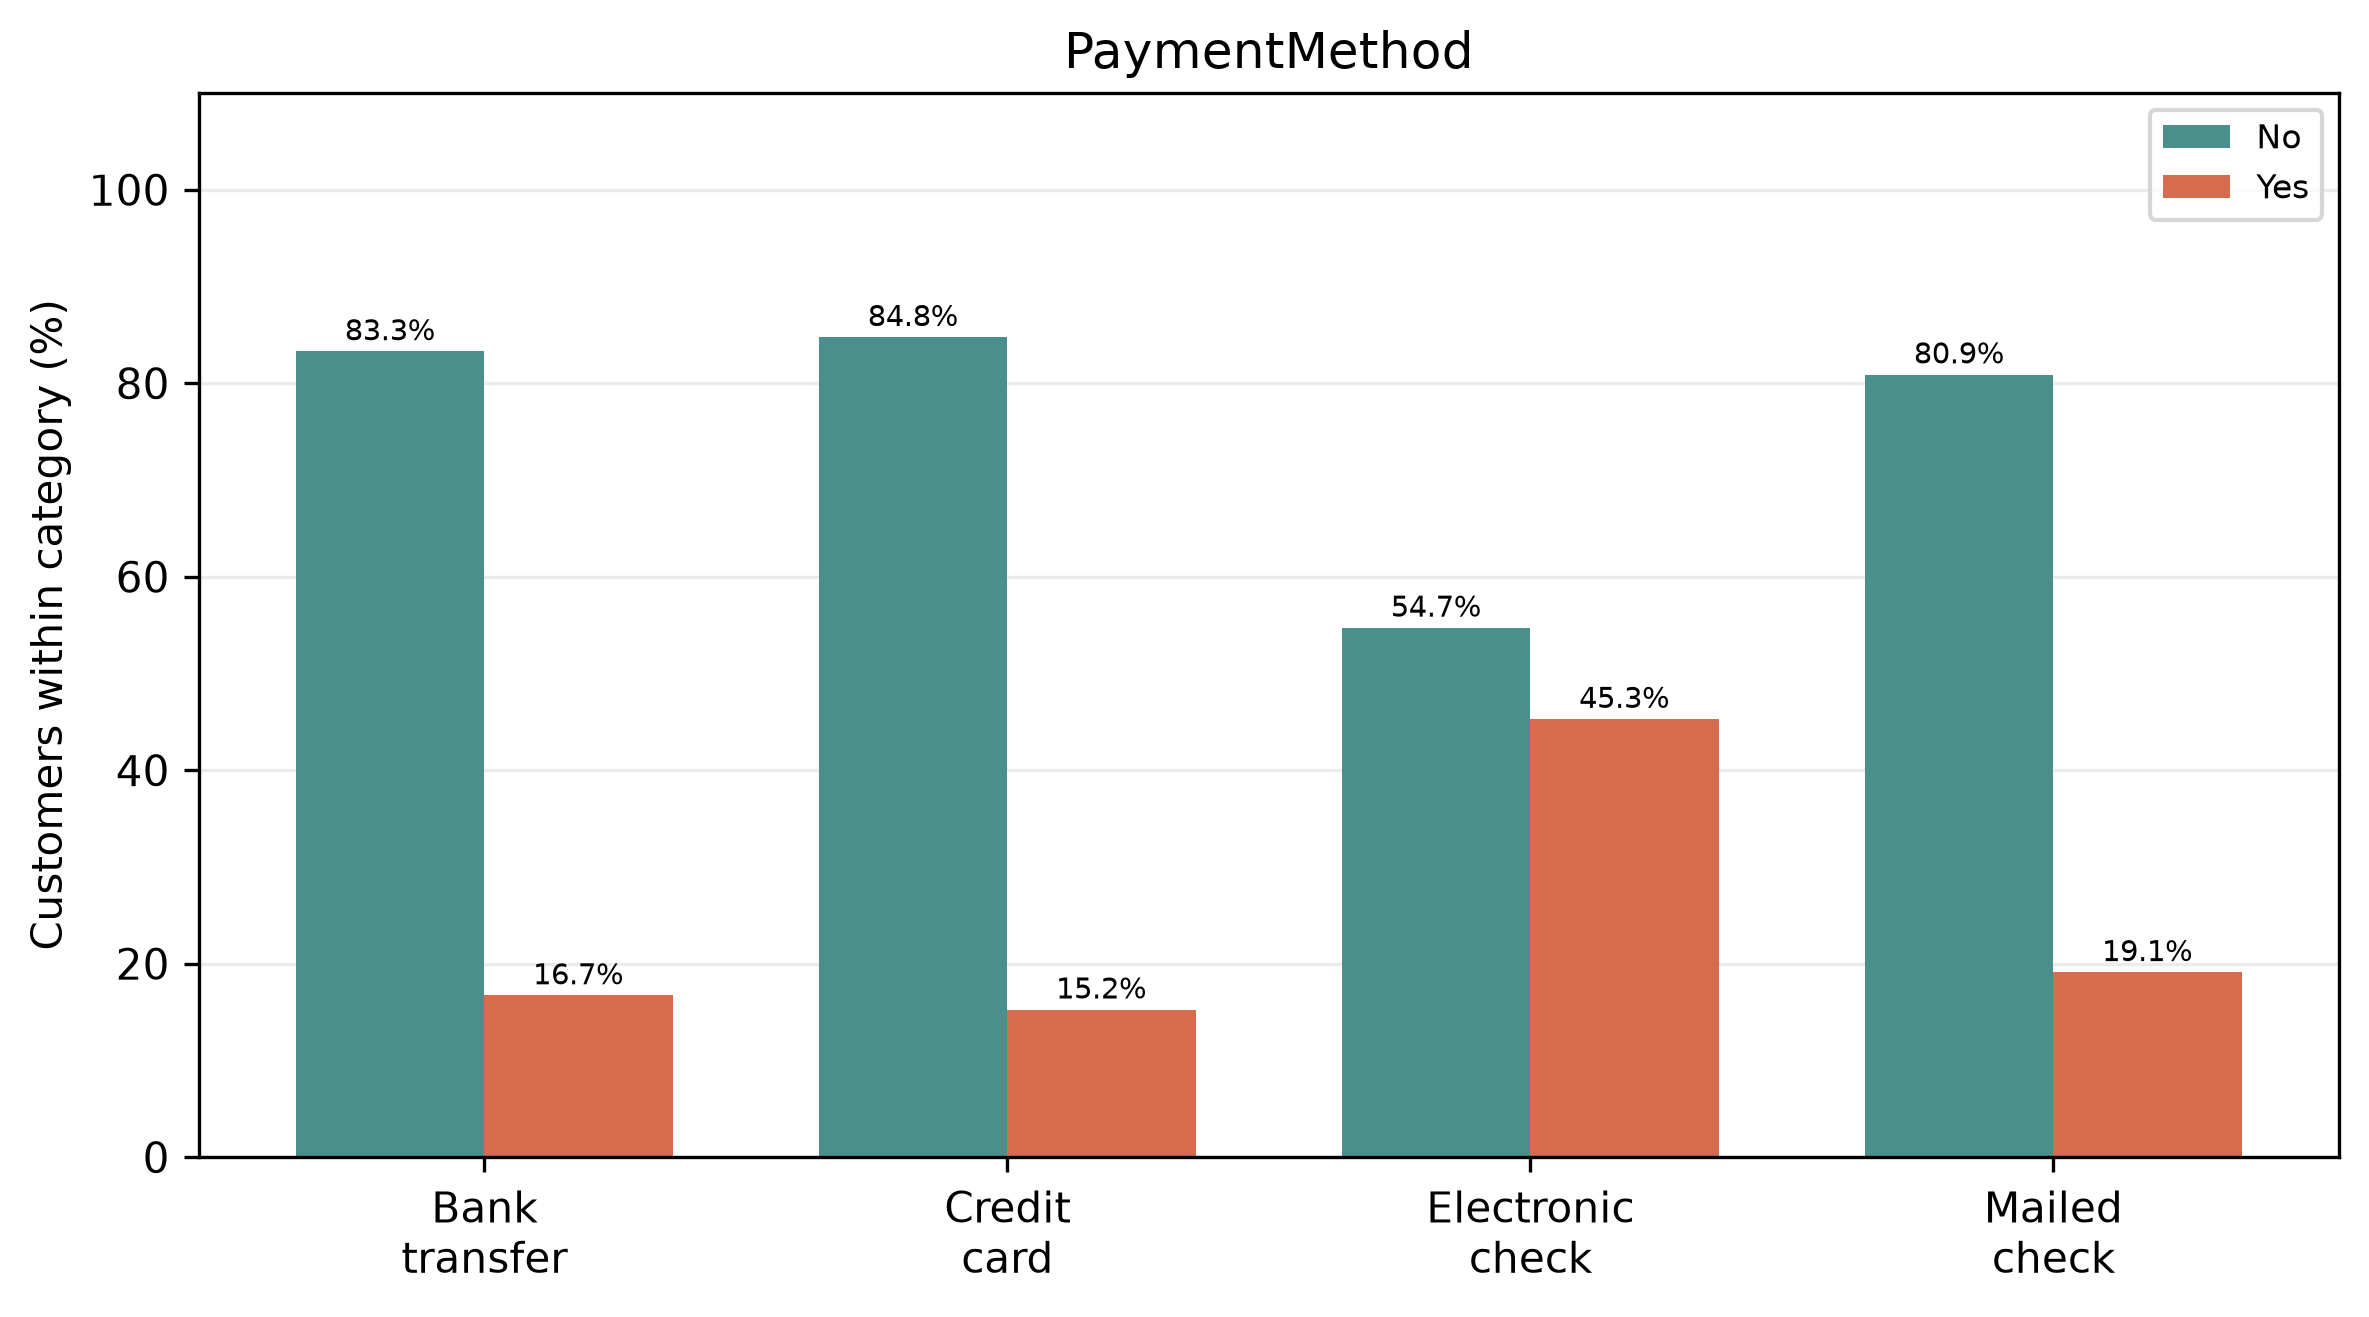
\includegraphics[width=0.95\textwidth]{../graphics/churn_categorical_relationships_06_payment_method.png}
\caption{\centering Churn rates by payment method.}
\label{fig:churn-categorical-payment-method}
\end{figure}


\section{Preprocessing Pipeline}

The preprocessing pipeline is implemented by the preprocessing telco file. Consist in a Class with methods Methods that allow realise the preprocessing.
This structure allow separate each step in the processing of data and is possible add steps simply adding methods to the class. 
No data augmentation is applied because the nature of the dataset not has images, isn´t necessary this technique.

\subsection{Format Standardization}
The pipeline selects the customer and service features used for modeling and excludes 
\texttt{customerID}, since it uniquely identifies each row and does not describe customer behavior. 
Categorical inputs remain in their original form until after splitting, when they are encoded using the training feature schema.

\subsection{Missing Data Handling}
\texttt{TotalCharges} is converted to numeric values using imputing. Its 11 blank entries in this dataset belong 
to customers with zero months of tenure, so they are imputed as zero. 
The target \texttt{Churn} is mapped to binary values, with \texttt{No}=0 and \texttt{Yes}=1. 
Any remaining rows with missing values are removed, but in this dataset there isn't that case because the 11 problematic samples where imputed. 
For the current dataset, all 7,043 rows remain after this step.

\subsection{Feature Engineering}
Two customer-level features are added. 
\texttt{NewCustomer} is set to 1 when tenure is zero and 0 otherwise.
\texttt{AvgMonthlyCharges} is calculated as total charges divided by tenure for existing customers; it is set to zero when tenure is zero to avoid division by zero.

\subsection{Train, Validation, and Test Split}
The data is split before fitting the categorical encoder or scaler. A stratified split with random seed 42 assigns 70\% of the records to training and divides the remaining 30\% equally between validation and test, yielding approximately 70\%/15\%/15\%. Stratification preserves the target class proportions in each subset. The validation arrays are available as \texttt{X\_validation} and \texttt{y\_validation} on the preprocessing object.

\subsection{Encoding, Normalization, and Scaling}
After splitting, categorical features are converted to one-hot indicators with \texttt{OneHotEncoder}. The encoder uses \texttt{handle\_unknown=ignore} so unseen categories can be transformed using the training feature schema. The encoder and \texttt{StandardScaler} are fitted using training data only, then applied unchanged to validation and test data to prevent information leakage. Standard scaling is applied to the continuous features \texttt{tenure}, \texttt{MonthlyCharges}, \texttt{TotalCharges}, and \texttt{AvgMonthlyCharges}. The binary \texttt{SeniorCitizen} feature and one-hot indicator columns are not scaled.

\subsection{Saved Splits}
The transformed train, validation, and test arrays, their target labels, and the feature names are saved in compressed NumPy format at \path{data/telco_preprocessed_splits.npz}. The \texttt{preprocess()} method continues to return \texttt{X\_train}, \texttt{X\_test}, \texttt{y\_train}, and \texttt{y\_test} for compatibility with the existing model notebooks; the validation split is available as attributes and in the saved file.

\section{Models}

All four models below share the exact same experimental protocol, so that any difference in the final numbers can be attributed to the algorithm itself and not to inconsistencies in how it was trained or measured. Each model is developed in its own notebook under \path{src/w1_supervized_learning/models/}, consumes the identical train/validation/test arrays produced by \texttt{PreprocessingTelco}, and follows the same four stages: a hyperparameter search driven by Optuna's tree-structured Parzen estimator sampler with median pruning \cite{akiba2019optuna}, a decision-threshold search performed strictly on held-out predictions, a single refit on the full training split, and one evaluation on the test split. The test set is deliberately touched only once per model, at the very end, so that none of the reported numbers have been used, even indirectly, to make a modeling decision.

The search itself never optimizes accuracy. With 73.5\% of customers staying, a model that always predicts ``no churn'' is already 73.5\% accurate while being completely useless for retention purposes, so accuracy would reward the wrong behaviour during tuning. Instead, every search optimizes average precision, the area under the precision--recall curve, which is the metric of choice for imbalanced classification problems because it is sensitive to how well the model ranks the minority class rather than to how many labels happen to match \cite{davis2006precision}. Only after the best configuration is found is a decision threshold chosen, by scanning candidate cut-off points and keeping the one that maximizes F1 on validation-style predictions the model has not been directly fit to.

Table~\ref{tab:hyperparameters} lists the winning configuration found for each model. A pattern is already visible before looking at a single test metric: every search converged on a comparatively small, heavily regularized model rather than the largest one it was allowed to try. That is usually a sign that the extra capacity had nothing useful left to fit, a point the Results and Discussion section returns to.

\begin{table}[H]
\centering
\small
\begin{tabular}{ll}
\toprule
\textbf{Model} & \textbf{Selected configuration} \\
\midrule
Logistic Regression & \texttt{penalty}=L2, \texttt{C}$\approx$0.40, no class weighting \\
Random Forest & \texttt{n\_estimators}=150, \texttt{max\_depth}=10, \texttt{min\_samples\_leaf}=8, \texttt{max\_features}=sqrt \\
XGBoost & \texttt{n\_estimators}=200, \texttt{learning\_rate}$\approx$0.043, \texttt{max\_depth}=3, \texttt{reg\_alpha}$\approx$7.4 \\
Neural Network (MLP) & 1 hidden layer of 48 units, dropout=0.35, batch normalization, 20 epochs \\
\bottomrule
\end{tabular}
\caption{\centering Winning hyperparameter configuration per model, found with a 50-trial (30 for the MLP) Optuna search.}
\label{tab:hyperparameters}
\end{table}

\subsection{Logistic Regression}
The linear model exists to answer a simple question: how much do the more elaborate models actually buy the project? Its search space covered L1, L2, and elastic-net penalties together with the inverse regularization strength \texttt{C}, and the winner was a fairly conservative L2 penalty with \texttt{C}$\approx$0.40, meaning the search preferred to keep coefficients modest rather than let the model chase every fluctuation in the training data. Because every input was standardized beforehand, the resulting coefficients are directly comparable, and the largest ones line up with exactly the features that stood out earlier in the churn-relationship charts: contract length, tenure, and internet service type. The fact that a model with no interaction terms and no non-linearities lands so close to the ensembles below is itself an early hint about how much signal this dataset actually contains.

\subsection{Random Forest}
The forest searched over the number of trees, their maximum depth, the minimum samples required to split or to form a leaf, the feature-sampling strategy, and the split criterion \cite{breiman2001randomforests}. The winning configuration used only 150 trees capped at depth 10, with a comparatively large minimum leaf size of 8. A Random Forest is not prone to overfitting simply by adding more trees, so if deeper, more numerous trees had helped, the search had every opportunity to pick them; instead it settled for a shallow, small forest, which again suggests the ceiling on this problem is set by the data rather than by the model's capacity.

\subsection{XGBoost}
Gradient boosting builds trees sequentially, each one correcting the residual errors of the ones before it, which in principle lets it capture more subtle patterns than bagging \cite{chen2016xgboost}. The search here covered ten hyperparameters at once, and the winning combination is telling: trees limited to depth 3, a cautious learning rate of about 0.043 spread over 200 boosting rounds, a strong L1 penalty (\texttt{reg\_alpha}$\approx$7.4) discouraging large leaf weights, and both row and column subsampling turned on. Every one of those choices dampens the model rather than empowering it. Interestingly, the search also settled on a \texttt{scale\_pos\_weight} of about 1.33, well below the dataset's true 2.77:1 imbalance ratio, meaning it found that correcting only partly for the imbalance, rather than fully rebalancing the loss, produced better-ranked probabilities.

\subsection{Neural Network (MLP)}
The multilayer perceptron is the only model built from scratch rather than imported from scikit-learn, using PyTorch \cite{paszke2019pytorch} for both the architecture and the training loop. Optuna was allowed to search over one to four hidden layers of 16 to 128 units each, dropout, batch normalization, the learning rate, weight decay, the number of epochs, and the batch size. Out of that considerably larger design space, the winning network has a single hidden layer of 48 units (a 47$\rightarrow$48$\rightarrow$1 architecture), trained for only 20 epochs with dropout of 0.35. Given four layers and 128 units per layer were on the table, the network choosing the smallest allowed footprint is the clearest version of the pattern already seen in the two tree-based models: more capacity was available, and it was not used, because there was nothing more to learn from these 47 encoded features.

\section{Results and Discussion}

\subsection{Head-to-head comparison}
Table~\ref{tab:model-comparison} reports every model's performance on its held-out test data, evaluated exactly once. Random Forest and XGBoost are effectively tied for the best average precision (0.672 and 0.671), Logistic Regression is a close third (0.658) despite being by far the simplest model, and the neural network trails the other three (0.631). No model reaches an accuracy of 80\%, and the gap between the best and worst F1 score is under two points -- the four models, built on genuinely different principles, all landed in nearly the same place. This lines up with the broader body of applied research on telecom churn prediction, where tree ensembles and linear baselines built on similar tabular features are consistently reported as strong, closely-matched performers \cite{ahmad2019}.

\begin{table}[H]
\centering
\small
\begin{tabular}{lrrrrrr}
\toprule
\textbf{Model} & \textbf{Avg. Precision} & \textbf{ROC-AUC} & \textbf{F1} & \textbf{Recall} & \textbf{Precision} & \textbf{Accuracy} \\
\midrule
Logistic Regression & 0.658 & 0.845 & 0.631 & 0.758 & 0.541 & 0.764 \\
Random Forest        & \textbf{0.672} & 0.841 & 0.623 & 0.673 & 0.580 & \textbf{0.783} \\
XGBoost              & 0.671 & \textbf{0.844} & \textbf{0.630} & 0.705 & 0.569 & 0.780 \\
Neural Network       & 0.631 & 0.843 & 0.625 & \textbf{0.757} & 0.532 & 0.759 \\
\bottomrule
\end{tabular}
\caption{\centering Test-set performance for all four models, each evaluated once on its held-out fold at its own tuned decision threshold.}
\label{tab:model-comparison}
\end{table}

The confusion matrices in Table~\ref{tab:confusion-summary} make the trade-off concrete. Logistic Regression and the neural network both catch around three out of every four churners (recall $\approx$0.76) but pay for it with more false alarms, while Random Forest is the most conservative model, missing more churners but rarely flagging a loyal customer by mistake. In a real retention campaign this is exactly the dial a business would want to turn: recall matters more when a retention offer is cheap, precision matters more when it is expensive, and the fact that four different algorithms land on four different points along that same trade-off, rather than one model dominating every column, says as much about the ceiling in the data as it does about any single model.

\begin{table}[H]
\centering
\small
\begin{tabular}{lrrrrr}
\toprule
\textbf{Model} & \textbf{Test size} & \textbf{True neg.} & \textbf{False pos.} & \textbf{False neg.} & \textbf{True pos.} \\
\midrule
Logistic Regression & 1,057 & 595 & 181 & 68 & 213 \\
Random Forest        & 1,057 & 639 & 137 & 92 & 189 \\
XGBoost              & 1,057 & 626 & 150 & 83 & 198 \\
Neural Network       & 1,409$^{*}$ & 786 & 249 & 91 & 283 \\
\bottomrule
\end{tabular}
\caption{\centering Confusion matrix for each model on its own test fold. $^{*}$See the testing note below regarding the neural network's fold size.}
\label{tab:confusion-summary}
\end{table}

\subsection{On testing and reproducibility}
No automated test suite (\texttt{pytest} or otherwise) exists yet for this workshop, which the team considers the most important gap to close before the next delivery. In its place, three weaker but real safeguards are already at work. First, all four notebooks import the same \texttt{PreprocessingTelco} class, so a bug in feature engineering or encoding would affect every model identically rather than silently favouring one of them. Second, the 5-fold stratified cross-validation used during every hyperparameter search is, in effect, twenty-five repeated end-to-end runs of the whole pipeline (five folds across fifty trials), and a broken step would have shown up as a crashed trial or a wildly inconsistent score rather than a clean result. Third, every random seed is fixed, so the numbers in this report are reproducible rather than a lucky draw.

That said, preparing this section surfaced a real inconsistency that a proper test would have caught automatically: the neural network notebook was executed before the preprocessing pipeline's split ratios were finalized, so its cached test fold has 1,409 rows (20\% of the data) instead of the 1,057 rows (15\%) shared by the other three models. The metrics in Table~\ref{tab:model-comparison} are each internally consistent, and the four models remain comparable in relative terms, but the neural network's exact test numbers should be treated as provisional until that notebook is re-run against the current pipeline. This is precisely the kind of drift a small assertion on split sizes would have flagged the moment it happened, and it is now the first unit test on the team's list.

\subsection{What the correlations in the graphics are really showing}
The EDA figures were built to compare each feature with the churn target one at a time, but looking across several of them side by side tells a more interesting story: many of these ``independent'' features are not independent at all, and that overlap is a large part of why every model above lands in the same narrow band of performance.

The clearest example sits in Figures~\ref{fig:churn-categorical-internet-security} and \ref{fig:churn-categorical-protection-support}. OnlineSecurity, OnlineBackup, DeviceProtection, TechSupport, StreamingTV, and StreamingMovies each get their own chart, yet all six repeat almost exactly the same shape: customers with no internet service churn at about 7.4\%, customers who have internet but skipped the add-on churn at roughly 40\%, and customers who took the add-on churn somewhere in between. That is not six separate warning signs; it is the same underlying fact -- whether a customer subscribes to internet service at all, and how invested they are in it -- echoed six times through six differently named columns. A model does not gain six times the information from these variables; realistically it gains one strong signal wrapped in five correlated copies of itself.

A second, related pattern connects contract type, payment method, and tenure. Month-to-month customers churn at 42.7\% against 2.8\% for two-year contracts (Figure~\ref{fig:churn-categorical-streaming-contract}), and electronic check is both the only payment method above a 20\% churn rate (45.3\%, Figure~\ref{fig:churn-categorical-payment-method}) and, in practice, the payment method most associated with exactly the same short-contract, low-tenure customers. These three variables read as three independent risk factors, but they largely describe one recognizable group of newer, less-committed subscribers seen from three different angles, which is why adding a fourth or fifth correlated variable rarely moves a model's score by much.

The numeric relationships tell the same story from a different direction. The tenure and MonthlyCharges boxplots (Figure~\ref{fig:churn-numeric-relationships}) show churners with a noticeably lower median tenure (10 months against 38) and higher median monthly charges (about 80 against 64), which is a genuine, usable signal -- it is exactly what both the linear model's coefficients and the tree-based models' feature importances lean on most heavily. But the boxes overlap substantially: plenty of customers who stay have 15--29 months of tenure and \$56--88 in monthly charges, which is precisely the range where most churners also sit. There is no tenure or spending threshold that cleanly separates the two groups; there is only a region where churn becomes more likely, not certain.

Put together, this is the honest answer to why none of the four models crossed 80\% accuracy or came close to it on any other metric. Three things compound against a higher ceiling: the target itself is imbalanced enough that a model gets 73.5\% accuracy for free just by refusing to predict churn, so the 76--78\% actually observed represents a real but modest lift, not a large one; the strongest predictors are correlated with each other rather than independent, so the model effectively has three or four usable signals dressed up as twenty columns instead of twenty genuinely different ones; and even those strongest signals overlap heavily between the two classes, so a meaningful share of customers are, on paper, indistinguishable regardless of which algorithm looks at them. That last point is confirmed by the hyperparameter search itself: Logistic Regression chose a moderate \texttt{C}, Random Forest stopped at a modest depth of 10, XGBoost preferred trees only three levels deep, and the neural network kept to a single 48-unit layer, even though every one of those searches was free to pick something larger. Four different algorithms, given the freedom to grow as complex as they wanted, all decided that more complexity was not worth it. That is a property of the dataset, not a shortcoming of any one model, and it sets a realistic, well-earned baseline for the deep sequential models the team will build in Workshop 2.

\section{Conclusion}
Workshop 1 set out to build a trustworthy supervised-learning baseline for churn prediction, and that goal was met. A preprocessing pipeline that splits before fitting anything, avoiding the leakage present in earlier drafts, now underpins a full exploratory analysis and four independently tuned models -- Logistic Regression, Random Forest, XGBoost, and a small PyTorch neural network -- compared under one identical protocol: the same data splits, the same search objective, and a single, honestly held-out evaluation. Random Forest and XGBoost lead on average precision, the linear baseline is a close and far more interpretable third, and the neural network, while competitive, did not benefit from the deeper architectures Optuna was free to try. That last result is itself useful: it says the team should not expect Workshop 2's more sequential architectures to outperform this baseline by a wide margin unless they bring in information this feature set does not currently contain.

The work was successful not because any single model produced an outstanding number, but because the project can now explain, with evidence from the data itself, why none of them did: a moderately imbalanced target, a set of predictors that are more correlated with each other than the column count suggests, and genuine overlap between the two classes in the strongest available features. That explanation, more than any single metric, is what makes this baseline usable going forward. The most immediate open items are to add an automated test suite that would have caught the neural network's stale test-fold size on its own, to re-run that notebook against the finalized preprocessing pipeline, and to consider a business-driven decision threshold -- built on the estimated cost of a missed churner versus a wasted retention offer, an approach with a track record in the churn literature \cite{verbeke2012} -- rather than the F1-optimal one used here. Extending the feature set with account-level interactions, or revisiting the imbalance with a technique such as SMOTE \cite{chawla2002smote} instead of scale-based weighting, are the most promising next steps for pushing past the ceiling this workshop uncovered.

\begin{thebibliography}{9}

\bibitem{ahmad2019}
Ahmad, A. K., Jafar, A., \& Aljoumaa, K. (2019). Customer churn prediction in telecom using machine learning in big data platform. \textit{Journal of Big Data}, 6, 28.

\bibitem{verbeke2012}
Verbeke, W., Dejaeger, K., Martens, D., Hur, J., \& Baesens, B. (2012). New insights into churn prediction in the telecommunication sector: A profit driven data mining approach. \textit{European Journal of Operational Research}, 218(1), 211--229.

\bibitem{breiman2001randomforests}
Breiman, L. (2001). Random forests. \textit{Machine Learning}, 45(1), 5--32.

\bibitem{chen2016xgboost}
Chen, T., \& Guestrin, C. (2016). XGBoost: A scalable tree boosting system. In \textit{Proceedings of the 22nd ACM SIGKDD International Conference on Knowledge Discovery and Data Mining} (pp. 785--794).

\bibitem{akiba2019optuna}
Akiba, T., Sano, S., Yanase, T., Ohta, T., \& Koyama, M. (2019). Optuna: A next-generation hyperparameter optimization framework. In \textit{Proceedings of the 25th ACM SIGKDD International Conference on Knowledge Discovery \& Data Mining} (pp. 2623--2631).

\bibitem{paszke2019pytorch}
Paszke, A., Gross, S., Massa, F., Lerer, A., Bradbury, J., Chanan, G., Killeen, T., Lin, Z., Gimelshein, N., Antiga, L., Desmaison, A., Kopf, A., Yang, E., DeVito, Z., Raison, M., Tejani, A., Chilamkurthy, S., Steiner, B., Fang, L., Bai, J., \& Chintala, S. (2019). PyTorch: An imperative style, high-performance deep learning library. \textit{Advances in Neural Information Processing Systems}, 32.

\bibitem{chawla2002smote}
Chawla, N. V., Bowyer, K. W., Hall, L. O., \& Kegelmeyer, W. P. (2002). SMOTE: Synthetic minority over-sampling technique. \textit{Journal of Artificial Intelligence Research}, 16, 321--357.

\bibitem{davis2006precision}
Davis, J., \& Goadrich, M. (2006). The relationship between precision-recall and ROC curves. In \textit{Proceedings of the 23rd International Conference on Machine Learning} (pp. 233--240).

\end{thebibliography}

\end{document}
